\documentclass[ngerman
  ,numbers=noenddot % obsolete
  ,headsepline
  ,parskip=half*
  ,openany
  ,DIV=12
  ,fleqn % mv align to left
]{scrbook}
  %,12pt
  %,titelpage % unused
  %,biblography=totoc  % unused
  %,landscape,twocolumn
\usepackage[ngerman]{babel}
\usepackage[T1]{fontenc}
\usepackage[utf8]{inputenc}
%\usepackage[ansinew]{inputenc}
\usepackage{lmodern} %Type1-Schriftart für nicht-englische Texte

\setlength{\unitlength}{1mm}
\emergencystretch 2em

\usepackage{lscape} % alt: pdflscape
\usepackage{amsmath,amsthm,amssymb}
\usepackage{latexsym}
\usepackage{enumerate}
\usepackage{verbatim}
\usepackage{graphicx}

\allowdisplaybreaks

%\usepackage{thmbox}

%\usepackage{natbib}

\usepackage[automark]{scrpage2} % Headline styles
\usepackage[square,numbers]{natbib}


\pagestyle{scrheadings}
%A better solution would be to use typearea package.


% Section Numbers moved left out
%\usepackage{sectsty}
%\makeatletter\def\@seccntformat#1{%
  %\protect\makebox[0pt][r]{\csname the#1\endcsname\hspace{12pt}}}\makeatother

% semibold instead of bold
%\renewcommand{\bfdefault}{sb}

\renewcommand*{\thefootnote}{[\arabic{footnote}]}

% Zeichen
\usepackage{nicefrac}
\usepackage{mathrsfs}
\usepackage{stmaryrd}
%simplewick

\usepackage{tikz}
\usetikzlibrary{matrix,arrows,decorations.pathmorphing}

\numberwithin{equation}{chapter}
\numberwithin{figure}{chapter}

%%%%  Abkürzungsverzeichnis  %%%%%%%%%%%%%%%%%%%%%%%%%%%%%%%%%%%%%%%%
\usepackage{nomencl}
% Befehl umbenennen in abk
\let\abk\nomenclature
% Deutsche Überschrift
\renewcommand{\nomname}{Abkürzungsverzeichnis}
% Punkte zw. Abkürzung und Erklärung
\setlength{\nomlabelwidth}{.20\hsize}
\renewcommand{\nomlabel}[1]{#1 \dotfill}
% Zeilenabstände verkleinern
\setlength{\nomitemsep}{-\parsep}
\makenomenclature

%% BASH: makeindex main.nlo -s nomencl.ist -o main.nls

%%%%  Theoreme Styles  %%%%%%%%%%%%%%%%%%%%%%%%%%%%%%%%%%%%%%%%%%%%%%
\makeatletter

\theoremstyle{plain}% default
\newtheorem{thm}{Satz}[chapter]
%\newtheorem{thm}[satz]{Satz}
\newtheorem{lemma}[thm]{Lemma}
\newtheorem{lem}[thm]{Lemma}
\newtheorem{kor}[thm]{Korollar}
\newtheorem{prop}[thm]{Proposition}
\newtheorem{cor}[thm]{Korollar}

\theoremstyle{definition}
\newtheorem{defn}[thm]{Definition}
\newtheorem{conj}[thm]{Conjecture}
\newtheorem{exmp}[thm]{Beispiel}
\newtheorem{bsp}[thm]{Beispiel}

\theoremstyle{remark}
\newtheorem{rem}[thm]{Bemerkung}
\newtheorem{bem}[thm]{Bemerkung}
\newtheorem{note}[thm]{Notiz}
\newtheorem{case}{Fall}

%custom pdf-metadata
%\pdfinfo{
%/Title (Title)
%/Subject (Subject)
%/Author (Maximilian Huber)
%/Keywords (keywords) }

\usepackage[german]{varioref}
%\usepackage[nameinlink,german]{cleveref}
\usepackage[colorlinks=true,linkcolor=black]{hyperref}

%% Autoref Names %%%%%%%%%%%%%%%%%
%\crefname{lemma}{Lemma}{Lemmas}
%\crefname{equation}{Gleichung}{Gleichungen}
%\crefname{definition}{Definition}{Definitionen}
%\crefname{algorithmus}{Algorithmus}{Algorithmen}
%\crefname{kor}{Korollar}{Korollare}

%%%%  new Commands  %%%%%%%%%%%%%%%%%%%%%%%%%%%%%%%%%%%%%%%%%%%%%%%%%
\def\bme{\boldsymbol{e}}

\def\A{\ensuremath \mathbb{A}}
%\def\B{\ensuremath \mathbb{B}}
\def\C{\ensuremath \mathbb{C}}
%\def\D{\ensuremath \mathbb{D}}
%\def\E{\ensuremath \mathbb{E}}
%\def\F{\ensuremath \mathbb{F}}
%\def\G{\ensuremath \mathbb{G}}
%\def\H{\ensuremath \mathbb{H}}
\def\I{\ensuremath \mathbb{I}}
%\def\J{\ensuremath \mathbb{J}}
%\def\K{\ensuremath \mathbb{K}}
%\def\L{\ensuremath \mathbb{L}}
%\def\M{\ensuremath \mathbb{M}}
\def\N{\ensuremath \mathbb{N}}
%\def\O{\ensuremath \mathbb{O}}
%\def\P{\ensuremath \mathbb{P}}
%\def\Q{\ensuremath \mathbb{Q}}
\def\R{\ensuremath \mathbb{R}}
%\def\S{\ensuremath \mathbb{S}}
%\def\T{\ensuremath \mathbb{T}}
%\def\U{\ensuremath \mathbb{U}}
%\def\V{\ensuremath \mathbb{V}}
%\def\W{\ensuremath \mathbb{W}}
%\def\X{\ensuremath \mathbb{X}}
%\def\Y{\ensuremath \mathbb{Y}}
\def\Z{\ensuremath \mathbb{Z}}

%\def\cA{\ensuremath \mathcal{A}}
%\def\cB{\ensuremath \mathcal{B}}
\def\cC{\ensuremath \mathcal{C}}
\def\cD{\ensuremath \mathcal{D}}
%\def\cE{\ensuremath \mathcal{E}}
%\def\cF{\ensuremath \mathcal{F}}
%\def\cG{\ensuremath \mathcal{G}}
%\def\cH{\ensuremath \mathcal{H}}
%\def\cI{\ensuremath \mathcal{I}}
%\def\cJ{\ensuremath \mathcal{J}}
%\def\cK{\ensuremath \mathcal{K}}
%\def\cL{\ensuremath \mathcal{L}}
\def\cM{\ensuremath \mathcal{M}}
\def\cN{\ensuremath \mathcal{N}}
%\def\cO{\ensuremath \mathcal{O}}
\def\cP{\ensuremath \mathcal{P}}
%\def\cQ{\ensuremath \mathcal{Q}}
%\def\cR{\ensuremath \mathcal{R}}
%\def\cS{\ensuremath \mathcal{S}}
%\def\cT{\ensuremath \mathcal{T}}
%\def\cU{\ensuremath \mathcal{U}}
%\def\cV{\ensuremath \mathcal{V}}
%\def\cW{\ensuremath \mathcal{W}}
%\def\cX{\ensuremath \mathcal{X}}
%\def\cY{\ensuremath \mathcal{Y}}
%\def\cZ{\ensuremath \mathcal{Z}}

%\def\sA{\ensuremath \mathscr{A}}
%\def\sB{\ensuremath \mathscr{B}}
%\def\sC{\ensuremath \mathscr{C}}
%\def\sD{\ensuremath \mathscr{D}}
\def\sE{\ensuremath \mathscr{E}}
%\def\sF{\ensuremath \mathscr{F}}
%\def\sG{\ensuremath \mathscr{G}}
%\def\sH{\ensuremath \mathscr{H}}
%\def\sI{\ensuremath \mathscr{I}}
%\def\sJ{\ensuremath \mathscr{J}}
%\def\sK{\ensuremath \mathscr{K}}
%\def\sL{\ensuremath \mathscr{L}}
%\def\sM{\ensuremath \mathscr{M}}
%\def\sN{\ensuremath \mathscr{N}}
%\def\sO{\ensuremath \mathscr{O}}
%\def\sP{\ensuremath \mathscr{P}}
%\def\sQ{\ensuremath \mathscr{Q}}
%\def\sR{\ensuremath \mathscr{R}}
%\def\sS{\ensuremath \mathscr{S}}
%\def\sT{\ensuremath \mathscr{T}}
%\def\sU{\ensuremath \mathscr{U}}
%\def\sV{\ensuremath \mathscr{V}}
%\def\sW{\ensuremath \mathscr{W}}
%\def\sX{\ensuremath \mathscr{X}}
%\def\sY{\ensuremath \mathscr{Y}}
%\def\sZ{\ensuremath \mathscr{Z}}

%\renewcommand{\headrulewidth}{0.2pt}

\newcommand{\myhr}{\rule{0.3\textwidth}{1pt}}

\let\epsilon\varepsilon
\let\phi\varphi

\DeclareMathOperator{\modulo}{mod}
\DeclareMathOperator{\conv}{conv}
\DeclareMathOperator{\Cof}{Cof}
\DeclareMathOperator{\grad}{grad}
\DeclareMathOperator{\Id}{Id}
\DeclareMathOperator{\dist}{dist}
\DeclareMathOperator{\diam}{diam}
\DeclareMathOperator{\co}{co}
\DeclareMathOperator{\supp}{supp}
\DeclareMathOperator{\graph}{graph}
\DeclareMathOperator{\slopes}{slopes}
\DeclareMathOperator{\Ob}{Ob}
\DeclareMathOperator{\Mor}{Mor}

% specific:
\newcommand{\Dm}{{\cD\mbox{-Modul}}}

\newcommand{\Cfx}{{\mathbb C\llbracket x\rrbracket}}
\newcommand{\Cft}{{\mathbb C\llbracket t\rrbracket}}
\newcommand{\Cfu}{{\mathbb C\llbracket u\rrbracket}}
\newcommand{\Cfxl}{{\mathbb C (\!(x)\!)}}
\newcommand{\Cftl}{{\mathbb C (\!(t)\!)}}
\newcommand{\Cful}{{\mathbb C (\!(u)\!)}}

\makeatother

\newcommand{\overbox}[2]{\ensuremath\begin{array}[b]{c}%
\makebox[0pt]{\fbox{\scriptsize#2}}\\[-2pt]\text{\small$\downarrow$}\\[-3pt]%
{\displaystyle#1}\end{array}}%


\usepackage{xcolor}
\usepackage{color}
\usepackage{framed}

\newenvironment{fshaded}{%
\def\FrameCommand{\fcolorbox{framecolor}{shadecolor}}%
\MakeFramed {\FrameRestore}}%
{\endMakeFramed}

%\newenvironment{comment}{\definecolor{shadecolor}{rgb}{1,.6,.6}%
%\definecolor{framecolor}{rgb}{0,0,0}%
%\begin{fshaded}}{\end{fshaded}}

\renewcommand{\comment}{\definecolor{shadecolor}{rgb}{.8,.8,.8}%
\definecolor{framecolor}{rgb}{0,0,0}%
\fshaded}
\renewcommand{\endcomment}{\endfshaded}

%Zeilenhöhe, für bessere lesbarkeit
\linespread{1.3}

\cfoot{-\thepage-\\\today}
\setboolean{@twoside}{false} 

%\usepackage{showframe}


\begin{document}

%TODO: set titel variable??

%%%%%%%%%%%%%%%%%%%%%%%%%%%%%%%%%%%%%%%%%%%%%%%%%%%%%%%%%%%%%%%%%%%%%
\frontmatter

%TODO; titelpage bitte nicht seitlich versetzt
\begin{titlepage}
  \thispagestyle{empty}
  \newcommand{\Rule}{%
    \textcolor{black}{\rule{\textwidth}{0.5mm}}%
  }
  \begin{center}\sffamily
    \normalfont\sffamily\large
    Bachelorarbeit
    %\vfill
    \Rule
    \vspace{5mm}
    \Huge{Explizite Berechnung der Levelt-Turrittin-Zerlegung für spezielle
      $\cD$-Moduln}
    %{Explizite Berechnung der Levelt-Turrittin-Zerlegung einer Klasse
      %von Fourier-Transformationen}
    \vspace{1mm}
    \Rule
  \end{center}
    %\vfill
    \normalfont\sffamily\large vorgelegt von \Large Maximilian Huber\\
    \normalfont\sffamily\large am            \Large Institut für Mathematik\\
    \normalfont\sffamily\large der           \Large Universität Augsburg\\
    \normalfont\sffamily\large betreut durch \Large Prof. Dr. Marco Hien\\
    \normalfont\sffamily\large abgegeben am  \Large 04.07.2013\\
    \vfill
    \vfill
\end{titlepage}
% vim: set ft=tex :


%\begin{center}
  %\today
%\end{center}
\tableofcontents{}
%\printnomenclature

%\newpage

\chapter{Einleitung}

Das in dieser Arbeit am meisten betrachtete Objekt, sind die meromorphen
Zusammenhänge (siehe Kapitel \ref{chap:meromZsh}). Diese sind eine algebraische
Sichtweise der allseits bekannten Systemen von gewöhnlichen
Differentialgleichungen. 

Des weiteren werden holonome lokalisierte $\cD$-Moduln eingeführt, diese sind
in $1:1$ Korrespondenz zu den meromorphen Zusammenhängen und werden in dieser
Arbeit immer verwendet, da sich mit diesen leichter Rechnen lässt.

\begin{comment}
Riemann-Hilbert-Korrespondenz:
\begin{center}
\begin{tikzcd}
  \left\{ \text{Regulär singuläre holonome $\cD$-Moduln}} \right\}\arrow{r} &
  \left\{ \text{Perverse Garben} \right\} \\
  \left\{ \text{Regulär singuläre meromorphe Zusammenhänge} \right\}
  \arrow[hookrightarrow]{u} \arrow{r} & 
  \left\{ \text{Lokale Systeme} \right\}
\end{tikzcd}
\end{center}
Vergleiche hierzu \cite[Sec 6]{REFKashiwara1984}.
Dies ist ein bekanntes Resultat über regulär singuläre meromorphe
Zusammenhänge, jedoch lässt sich diese Aussage nicht auf irregulär singuläre
meromorphe Zusammenhänge fortsetzen.
\end{comment}

\begin{comment}
Ziel der Arbeit
\end{comment}
\begin{comment}
In dieser Arbeit soll zunächst die Theorie der meromorphen Zusammenhänge
eingeführt werden.
\end{comment}

\begin{comment}
Vorraussetzungen
\end{comment}
Es wird in dieser Arbeit kein Vorwissen über $\cD$-Moduln bzw. meromorphe
Zusammenhänge vorausgesetzt, diese beiden Begriffe werden in den ersten Zwei
Kapiteln eingeführt.

\begin{comment}
Aufbau / inhalt der Kapitel
\end{comment}
Im ersten Kapitel wird die Theorie der $\cD$-Moduln eingeführt.

Im zweiten Kapitel werden die meromorphen Zusammenhänge definiert, diese sind
das wichtigste Objekt, das in dieser Arbeit diskutiert werden soll.
Ein wichtiges Resultat, in diesen Kapiteln, ist die Äquivalenz von meromorphen
Zusammenhängen zu holonomen lokalisierten $\cD$-Moduln, da man mit letzteren
gut rechnen kann.

Das dritte Kapitel beschäftigt sich ausschließlich mit Operationen auf
meromorphen Zusammenhängen.
Vorgestellt werden Tensorprodukt, Pullback und Pushforward,
Fouriertransformation, die sogenannte Betrachtung bei Unendlich und das Twisten
eines meromorphen Zusammenhangs.

Im vierten Kapitel soll das Levelt-Turrittin-Theorem vorgestellt werden, 
welches Nützlich ist, um die Stokes Struktur eines 

\begin{comment}
Die Levelt-Turrittin-Theorem ist eine sogenannte Slope-Filtration. Diese
Klasse, der Slope-Filtrationen wird in \cite{0812.3921} betrachtet.
\end{comment}

Das letzte Kapitel wird die Levelt-Turrittin-Zerlegung auf eine Klasse von
meromorphen Zusammenhängen angewendet. Dazu wird zu Beginn ein Rezept gegeben,
welches die gewünschten Zusammenhänge beschreibt. Zu diesen Zusammenhängen
werden zunächst allgemeine Aussagen getroffen bevor in Abschnitt
\ref{sec:LT-speziell} ganz konkret eine Levelt-Turrittin-Zerlegung zu einem
meromorphen Zusammenhang berechnet wird.

\begin{comment}
Ich möchte diesen Zeitpunkt nutzen, um Herrn Prof. Dr. Hien dafür zu danken,
das er mir ermöglicht hat, mich mit diesem Thema zu beschäftigen.
Auch bedanke ich mich für die hervorragende Betreuung, welche diese Arbeit erst
ermöglicht hat.
\end{comment}

% vim:set ft=tex foldmethod=marker foldmarker={{{,}}}:


\mainmatter
%%%%%%%%%%%%%%%%%%%%%%%%%%%%%%%%%%%%%%%%%%%%%%%%%%%%%%%%%%%%%%%%%%%%%
%\part{Theorie}

%!TeX root = main.tex
\chapter{Mathematische Grundlagen}

\begin{comment}
Hier werde ich mich auf \cite{sabbah_cimpa90} und \cite{coutinho1995primer}
beziehen.
\end{comment}

Wir betrachten $\C$ hier als Complexe Mannigfaltigkeit mit der Klassischen
Topologie.
In dieser Arbeit spielen die folgenden Funktionenräume eine große Rolle:
\begin{itemize}
\item $\C[x]:=\{ \sum^{N}_{i=1}a_ix^i | N\in \N \}$ die einfachen Potenzreihen
\item $\C\{x\}:=\{ \sum^{\infty}_{i=1}a_ix^i | \mbox{pos.
  Konvergenzradius} \}=(\cO_{\C})_0$ die formalen Potenzreihen mit positivem
Konvergenzradius (\cite[Chap 5.1.1]{hotta2007d})
\item $\C\llbracket x\rrbracket:=\{ \sum^{\infty}_{i=1}a_ix^i \}$ die formalen
Potenzreihen
\item $K:=\Ckxl:=\C\{x\}[x^{-1}]$ der Ring der Laurent Reihen.
\item $\hat{K}:=\Cfxl:=\C\llbracket x\rrbracket[x^{-1}]$ der Ring der
formalen Laurent Reihen.
\item $\tilde\cO$ als der Raum der Keime aller (möglicherweise mehrdeutigen)
Funktionen. (bei \cite{hotta2007d} mit $\tilde K$ bezeichnet)
\end{itemize}
Wobei offensichtlich die Inclulsionen $\C[x]\subsetneq\C\{x\}\subsetneq\Cfx$ und
$K\subsetneq\hat K$ gelten.

\begin{comment}
Es bezeichnet der Hut ($ \, \hat \,\, $) das jeweils formale äquivalent zu
einem konvergentem Objekt.
\end{comment}

\begin{comment}
\begin{lem}[Seite 2]
ein paar eigenschaften
\begin{enumerate}
\item $\C[x]$ ist ein graduierter Ring, durch die Grad der
Polynome. Diese graduierung induziert eine aufsteigende Filtrierung.

alle Ideale haben die form $(x-a)$ mit $a\in \C$
\item wenn $\mathfrak{m}$ das maximale Ideal von $\C[x]$ (erzeugt von
$x$ ist), so ist
\[
  \C[[x]]=
  \underset{k}{\underleftarrow{\lim}} \C[X]\backslash\mathfrak{m}^k
\]
The ring $\C[[x]]$ ist ein nöterscher lokaler Ring:
jede Potenzreihe mit konstantem term $\neq 0$ ist invertierbar.

Der ring ist ebenfalls ein diskreter ??? Ring (discrete valuation
ring)

Die Filtrierung nach grad des Maximalen Ideals, genannt
$\mathfrak{m}$-adische Fitration, ist die Filtrierung
$\mathfrak{m}^k=\{f\in \C[[x]]|v(f)\geq k\}$

und es gilt $gr_\mathfrak{m}(\C[[x]])=\C[x]$
\end{enumerate}
\end{lem}
\end{comment}

Für $v=(v_1,\dots,v_n)$ ein Vektor, bezeichnet 
\[
\,^tv:= \begin{pmatrix}
  v_{1}\\
  \vdots\\
  v_{n}
\end{pmatrix}
\]
den Transponierten Vektor. Es bezeichnet $M(n\times m,k)$ die Menge der $n$ mal
$m$ Dimensionalen Matritzen mit einträgen in $k$.

\begin{defn}[Direkte Summe] \cite[4(Categories).5.1]{stacks-project}
Seien $x,y\in \Ob(\cC)$, eine \emph{Direkte Summe} oder das \emph{coprodukt}
von $x$ und $y$ ist ein Objekt $x\oplus y\in \Ob(\cC)$ zusammen mit
Morphismen $i\in\Mor_\cC(x,x\oplus y)$ und $j\in\Mor_\cC(y,x\oplus y)$ so
dass die folgende universelle Eigenschaft gilt: für jedes $w\in Ob(\cC)$ mit
Morphismen $\alpha\in\Mor_\cC(x,w)$ und $\beta\in\Mor_\cC(y,w)$ existiert ein
eindeutiges $\gamma\in\Mor_\cC(x\oplus y,w)$ so dass das Diagram
\begin{center}
\begin{tikzpicture} [scale=3.3, descr/.style={fill=white,inner sep=2.5pt} ]
\matrix (m) [
  matrix of math nodes
  , row sep=2em
  , column sep=3em
  %, text height=3em
  %, text depth=0.25em
]{
    & y         &  &   \\
  x & x\oplus y &  &   \\
    &           &  & w \\
};
%TODO: Pfeile
\path[->,font=\scriptsize,>=angle 90]
(m-1-2) edge node[left]{$j$} (m-2-2)
(m-2-1) edge node[above]{$i$} (m-2-2)
(m-1-2) edge node[right]{$\beta$} (m-3-4)
(m-2-1) edge node[below]{$\alpha$} (m-3-4)
;
\path[->,font=\scriptsize,>=angle 90,dashed]
(m-2-2) edge node[above]{$\exists!\gamma$} (m-3-4)
;
\end{tikzpicture}
\end{center}
kommutiert.
\end{defn}

\begin{defn}[Tensorprodukt]
\cite[3(Algebra).11.21]{stacks-project}
\begin{comment}
Faserprodukt: \cite[4(Categories).6.1]{stacks-project}
\end{comment}
% von Vorlesung Algebra 2

\begin{center}
\begin{tikzpicture} [scale=3.3, descr/.style={fill=white,inner sep=2.5pt} ]
  \matrix (m) [
    matrix of math nodes
    , row sep=2em
    , column sep=3em
    %, text height=3em
    %, text depth=0.25em
  ]{
    M\times N & M\otimes_RN \\
              & T \\
  };
  %TODO: Pfeile
  \path[->,font=\scriptsize,>=angle 90]
  (m-1-1) edge node[above]{$  $} (m-1-2)
  (m-1-1) edge node[below]{$f$} (m-2-2)
  ;
  \path[->,font=\scriptsize,>=angle 90,dashed]
  (m-1-2) edge node[right]{$\exists!\gamma$} (m-2-2)
  ;
\end{tikzpicture}
\end{center}
\begin{comment}
Für eine Abbildung $f:M\rightarrow M'$ definiere das Tensorprodukt davon über
$R$ mit $N$ als
\[
\id_N \otimes f:
\begin{array}[t]{ccc}
N\otimes_{R}M & \rightarrow & N\otimes_{R}M'\\
n\otimes m & \mapsto & n\otimes f(m)
\end{array}
\]
\end{comment}
\end{defn}
\begin{bem} \label{bem:Rechenregeln-Tensorprodukt}
Hier ein paar Rechenregeln für das Tensorprodukt,
\begin{align}
(M\otimes_R N)\otimes_S L &\cong M\otimes_R (N \otimes_S L)
  \label{bem:Rechenregeln-Tensorprodukt1}\\
M\otimes_R R &\cong M \label{bem:Rechenregeln-Tensorprodukt2}
\end{align}
Sei $f:M'\rightarrow M$ eine Abbildung, so gilt
\begin{align}
N\otimes_R(M/\im(f)) &\cong N\otimes_R M / \im(\id_{R}\otimes f)
\label{bem:Rechenregeln-Tensorprodukt3}
\end{align}
\end{bem}
%TODO: tensorprodukt / faserprodukt zum basiswechsel

\begin{defn}[Exacte Sequenz]
Eine Sequenz
\begin{center}
\begin{tikzpicture} [scale=3.3, descr/.style={fill=white,inner sep=2.5pt} ]
  \matrix (m) [
    matrix of math nodes
    , row sep=2em
    , column sep=3em
    %, text height=3em
    %, text depth=0.25em
  ]{
    %M_0 
    & \cdots & M_{i-1} & M_i & M_{i+1} & \cdots & 
    %M_n 
  \\
  };
  %TODO: Pfeile
  \path[->,font=\scriptsize,>=angle 90]
  %(m-1-1) edge node[above]{$f_0$} (m-1-2)
  (m-1-2) edge 
    %node[above]{$f_{i-2}$} 
  (m-1-3)
  (m-1-3) edge node[above]{$f_{i-1}$} (m-1-4)
  (m-1-4) edge node[above]{$f_i$} (m-1-5)
  (m-1-5) edge 
    %node[above]{$f_{i+1}$} 
  (m-1-6)
  %(m-1-6) edge node[above]{$f_{n-1}$} (m-1-7)
  ;
\end{tikzpicture}
\end{center}
heißt exact, wenn für alle $i$ gilt, dass
$\im(f_{i-1})=\ker{f_i}$.
\end{defn}
\begin{defn}[Kurze exacte Sequenz]
Eine kurze exacte Sequenz ist eine Sequenz
\begin{center}
\begin{tikzpicture} [scale=3.3, descr/.style={fill=white,inner sep=2.5pt} ]
  \matrix (m) [
    matrix of math nodes
    , row sep=2em
    , column sep=3em
    %, text height=3em
    %, text depth=0.25em
  ]{
    0 & M' & M & M'' & 0 \\
  };
  %TODO: Pfeile
  \path[->,font=\scriptsize,>=angle 90]
  (m-1-1) edge node[above]{$  $} (m-1-2)
  (m-1-2) edge node[above]{$f$} (m-1-3)
  (m-1-3) edge node[above]{$g$} (m-1-4)
  (m-1-4) edge node[above]{$  $} (m-1-5)
  ;
\end{tikzpicture}
\end{center}
welche exact ist.
\end{defn}

\begin{defn}[Kokern]
Ist $f:M'\rightarrow M$ eine Abbildung, so ist der \emph{Kokern} von $f$
definiert als $\coker(f)=M/\im(f)$.
\end{defn}

\begin{prop}
Ist $f:M'\rightarrow M$ eine injektive Abbildung, so ist
\begin{center}
\begin{tikzpicture} [scale=3.3, descr/.style={fill=white,inner sep=2.5pt} ]
  \matrix (m) [
    matrix of math nodes
    %, row sep=2em
    , column sep=3em
    %, text height=3em
    %, text depth=0.25em
  ]{
    0 & M' & M & M/f(M')      & 0 \\
      &    & m & m \mod f(M') &   \\
  };
  %TODO: Pfeile
  \path[->,font=\scriptsize,>=angle 90]
  (m-1-1) edge (m-1-2)
  (m-1-2) edge node[above]{$f$} (m-1-3)
  (m-1-3) edge node[above]{$\pi$} (m-1-4)
  (m-1-4) edge (m-1-5)
  ;
  \path[|->,font=\scriptsize,>=angle 90]
  (m-2-3) edge (m-2-4)
  ;
\end{tikzpicture}
\end{center}
eine kuze exacte Sequenz.
\end{prop}
\begin{proof}
    
\end{proof}

\begin{defn}[Filtrierung] \label{defn:Filtrierung}
\cite[Def 10.13.1.]{stacks-project}
\cite[Rem 2.5.]{elliottDmod}
Eine \emph{aufsteigende Filtrierung $F$} von einem Objekt (Ring) $A$ ist eine
Familie von $(F_iA)_{i\in\Z}$ von Unterobjekten (Unterring), so dass 
\[ 0\subset\cdots\subset F_i\subset F_{i+1} \subset \cdots \subset A \]
und definiere weiter $gr_i^FA:=F_iA\slash F_{k-1}A$ und damit das zu $A$ mit
Filtrierung $F$ \embh{assoziierte graduierte Modul} 
\[gr^FA:=\bigoplus_{k\in\Z}gr_i^FA \,. \]
\begin{comment}
$gr_i^F$ als was??
\end{comment}
\end{defn}

\begin{defn}
\cite{ayoubIntro}
\cite[Def 3.2.1]{sabbah_cimpa90}
Eine Filtrierung heißt \emph{gut}, falls ...
\end{defn}

\begin{defn}[Kommutator]%zula seite 15
Sei $R$ ein Ring. Für $a,b\in R$ wird
\[[a,b]=a\cdot b-b\cdot a\]
als der \emph{Kommutator von a und b} definiert.
\end{defn}
% komutativ, dann immer kommutator gleich 0

\begin{prop} \label{prop:d-modul-komutator-regeln}
Sei $k\in \{ \C[x],\Ckx,\Cfx,K,\hat K \}$.
Sei $\partial_x:k\rightarrow k$ der gewohnte Ableitungsoperator
nach $x$, so gilt 
% geklaut aus Zula Barbara
\begin{enumerate}
\item $[ \partial_x,x] = \partial_xx-x\partial_x=1 $
%und damit ist $\cD_k$ insbesondere nicht kommutativ.
\item für $f\in k$ ist
\[ [\partial_x,f] = \frac{\partial f}{\partial x} \,. \]
\item Es gelten die Formeln\\
\begin{align*}
[\partial_x,x^k]   &= kx^{k-1}\\
[\partial_x^j,x]   &= j\partial_x^{j-1}\\
[\partial_x^j,x^k] &= \sum_{i\geq1}\frac{k(k-1)\cdots(k-i+1)
  \cdot j(j-1)\cdots(j-i+1)}{i!}x^{k-i}\partial_x^{j-i} \\
\end{align*}
\end{enumerate}
\end{prop}
\begin{proof}
\begin{enumerate}
\item Klar.
\item Für ein Testobjekt $g\in k$ ist
\[
[\partial_x,f]\cdot g=\partial_x(fg)-f\partial_xg=
  (\partial_xf)g+\underset{=0}{\underbrace{ 
  f(\partial_xg)-f(\partial_xg)}}=
  (\partial_xf)g
\]
\item Siehe \cite[???]{ZulaBarbara}
\end{enumerate}
\end{proof}

% vim: set ft=tex :

%\newpage

% In chapter "Meromorphe Zusammenhänge" verschoben
%% das gleiche wie Meromorphe zusammenhänge?

\section{\cD-Moduln}

\subsection{Lokalisierung eines $\C\{x\}$-Moduls}

\begin{defn}
  Sei $M$ ein $\C\{x\}$-Modul und $K=\C\{x\}[x^{-1}]$, dann ist die
  Lokalisierung
  \[ M[x^{-1}]:=M\otimes_{\C\{x\}}K \,. \]
\end{defn}

\subsection{Lokalisierung eines holonomen $\cD$-Moduls}

%vim: set ft=tex :

%\newpage

%!TeX root = main.tex
% TODO; wie darf ich einen Meromorphen verändern, (das P verändern) ohne das
% sich effektiv was ändert?
% TODO: \cM = \cM_K ... replace
% TODO: Dimension eines Meromorphen Zusammenhang
\chapter{Meromorphe Zusammenhänge}
\begin{comment}
Alle MeromZsh sind $\cD$-Moduln aber nicht andersherum?
\end{comment}

\section{Systeme von ODEs und Meromorphe Zusammenhänge}
%TODO: \tilde cO --> \tilde \cO
\cite[Chap 5.1.1]{hotta2007d} %abgeschrieben
Für eine Matrix $A(x)=(a_{ij}(x))_{ij}\in M(n\times n,K)$ betrachten wir das
System von gewöhnlichen Differentialgleichungen (kurz ODEs)
\begin{equation}
\label{eq:KlassischesODE}
%TODO: partial oder d
\frac{d}{dx}u(x)=A(x)u(x)
\end{equation}
wobei $u(x)=\,^t(u_1(x),\dots,u_n(x))$ ein Spaltenvektor von unbekannten
Funktionen. Wir werden (\ref{eq:KlassischesODE}) immer in einer Umgebung um
$x=0\in\C$ betrachten. Als Lösungen von (\ref{eq:KlassischesODE}) betrachten
wir Keime von holomorphen (aber möglicherweise mehrdeutigen)
 %but possibly multivalued auf
Funktionen an $x=0$ (geschrieben als $\tilde\cO$).
%auf der punktierten Scheibe
%$B_\epsilon^*=\{x\in\C|0<|x|<\epsilon\}$, wobei $\epsilon>0$ klein genug sei.
 Wir sagen $v(x)=\,^t(v_1(x),\dots,v_n(x))$ ist
eine Lösung von (\ref{eq:KlassischesODE}), falls $ v_i\in\tilde \cO$ für alle
$i\in\{1,\dots,n\}$ und $v$ die Gleichung (\ref{eq:KlassischesODE}),
auf einer Umgebung um die $0$, erfüllt.

\begin{comment}
TODO: zeige, das der lösungsraum die eigenschaften von $\cD$-Moduln erfüllt\\
siehe alternativer Zugang
\end{comment}

Nun wollen wir dieses Klassische Gebilde nun in die moderne Sprache der
Meromorphen Zusammenhänge übersetzen.

%\section{Meromorpher Zusammenhang (Definition)}
%Quelle ist \cite{sabbah_cimpa90}
\begin{defn}[Meromorpher Zusammenhang] \label{def:merom-zush}
Ein \emph{Meromorpher Zusammenhang} (bei $x=0$) ist ein Tuppel
$(\cM_K,\partial)$ und besteht aus folgenden Daten:
\begin{itemize}
\item $\cM_K$, ein endlich dimensionaler $K$-Vektor Raum
\item einer $\C$-linearen Abbildung $\partial:\cM_K\rightarrow \cM_K$,
genannt \emph{Derivation} oder \emph{Zusammenhang}, welche für alle $f\in K$
und $u\in \cM_K$ die \emph{Leibnitzregel}
\begin{equation}\label{eq:Leibnitzregel}
\partial(fu)=f'u+f\partial u %TODO: hier klammern um das letzte u ?
\end{equation}
erfüllen soll.
\end{itemize}
\end{defn}

\begin{defn}
Seien $(\cM_K,\partial_\cM)$ und $(\cN_K,\partial_\cN)$ zwei Meromorphe
Zusammenhänge. Eine $K$-lineare Abbildung $\phi:\cM\rightarrow\cN$ heißt
Morphismus von Meromorphen Zusammenhängen, falls sie
$\phi\circ\partial_\cM=\phi\circ\partial_\cN$ erfüllt. In diesem Fall schreiben
wir auch $\phi:(\cM_K,\partial_\cM)\rightarrow(\cN_K,\partial_\cN)$.
\end{defn}

\begin{bem}
\begin{enumerate}
\item Später wird man auf die Angabe von $\partial$ verzichten und einfach
$\cM_K$ als den Meromorphen Zusammenhang bezeichnen, auch wird manchmal auf die
Angabe von $K$ verzichtet.
\item \cite[Rem 5.1.2.]{hotta2007d}
Die Bedingung (\ref{eq:Leibnitzregel}) ist zur schwächeren Bedingung
\[
\partial(fu)=f'u+f\partial u \,,
\]
welche für alle $f\in \tilde\cO$ und für alle $u\in \cM_K$ erfüllt sein muss,
äquivalent.
\end{enumerate}
\end{bem}

\begin{defn}[Zusammenhangsmatrix] \cite[Seite 129]{hotta2007d}
Sei $(\cM_K,\partial)$ ein Meromorpher Zusammenhang so wähle eine $K$-Basis
$\{e_i\}_{i\in\{1,\dots,n\}}$ von $\cM$. Dann ist die
\emph{Zusammenhangsmatrix bzgl. der Basis $\{e_i\}_{i\in\{1,\dots,n\}}$} die
Matrix $A(x)=(a_{ij}(x))\in M(n\times n,K)$ definiert durch
%\[ \partial e_j=-\sum_{i=1}^na_{ij}(x)e_i \,. \]
\[ a_{ij}(x) = -^te_i \partial e_j \,. \]
\end{defn}

Also ist, bezüglich der Basis $\{e_i\}_{i\in\{1,\dots,n\}}$, die Wirkung von
$\partial$ auf $u=:\,^t(u_1,\dots,u_n)$ beschrieben durch
\[
\partial(u) = \partial \Big( \sum_{i=1}^nu_i(x)e_i \Big)
\overbox{=}{??}\sum_{i=1}^n \Big( u_i'(x)-
\sum_{j=1}^na_{ij}u_j(x) \Big)e_i \,.
\]
Einfache Umformungen zeigen, dass die Bedingung $\partial u(x)=0$, für
$u(x)\in \sum_{i=1}^n u_ie_i\in \tilde \cO \otimes_K\cM$, äquivalent zu der
Gleichung
\begin{equation*}
u'(x)=A(x)u(x)
\end{equation*}
für $u(x)=\,^t(u_1(x),\dots,u_n(x))\in\tilde \cO^n$. Damit haben wir gesehen,
dass jeder Meromorphe Zusammanhang $(\cM,\partial)$ ausgestattet mit einer
$K$-Basis $\{e_i\}_{i\in\{1,\dots,n\}}$ von $\cM$ zu einem ODE zugeordnet
werden kann.

Umgekehrt können wir für jede Matrix $A(x)=(a_{ij}(x))$ den
assoziierten Meromorphen Zusammenhang $(\cM_A,\partial_A)$ %TODO: improve notation
angeben, durch
\begin{align*}
\cM_A & :=\bigoplus_{i=1}^n Ke_i \,, & \partial_A e_i &:=
-\sum_{i=1}^na_{ij}(x)e_i \,.
\end{align*}

\begin{comment}
\section{Alternativer Zugang}
Hier wird nun ein alternativer Zugang, wie in \cite[3.1.1]{sabbah_cimpa90},
präsentiert. Sei $\cF$ ein Funktionenraum, auf dem die Differentialoperatoren
$\cD$ wirken.

Sei $P$ ein linearer Differentialoperator mit Koeffizienten in $a_i(t)\in\Ckx$
geschrieben als $P=\sum^{d}_{i=0}{a_{i}(t)\partial_t^i}$.
Man sagt eine Funktion $u\in\cF$ ist Lösung von $P$, falls $u$ die Gleichung
$Pu=0$ erfüllt.
Man sagt $0$ ist ein singulärer Punkt falls $a_d(0)=0$.
Falls $0$ kein singulärer Punkt ist, hat $P$ genau $d$ über $\C$ Unabhängige
Lösungen in $\C\{t\}$. %TODO: oder \tilde\cO

Falls $u$ ein Lösung von $P$ ist, so ist $u$ auch Lösung von $Q\cdot P$ mit
$Q\in \cD$. Also hängt die Lösung nur vom Links Ideal $I$ von $\cD$, welches
von $P$ erzeugt wird.
\end{comment}

\section{Eigenschaften}
%Hier nun einige Eigenschaften Meromorpher Zusammenhänge.
\begin{comment}
\cite[4.2]{sabbah_cimpa90}
Let $\cM$ be a left $\cD$-module. First we consider it only as a
$\C\{x\}$-module and let $\cM[x^{-1}]$ be the localized module.
\end{comment}

%TODO: reihenfolge bei sabbah anderst!!!
\begin{lem}[Lemma vom zyklischen Vektor] \label{lem:Zyklischer-Vektor}
\cite[Thm 4.3.3]{sabbah_cimpa90}
\cite[Satz 4.8]{ZulaBarbara}
Sei $\cM_K$ ein Meromorpher Zusammenhang. Es Existiert ein Element
$m\in\cM_K$ und eine ganze Zahl $d$ so dass
$m,\partial_xm,\dots,\partial_x^{d-1}m$ eine $K$-Basis von $\cM_K$ ist.
\end{lem}
\begin{proof}
\cite[Satz 4.8]{ZulaBarbara}
\end{proof}

\begin{thm}
\cite[Thm 4.3.2]{sabbah_cimpa90}
Ein Meromorpher Zusammenhang bestimmt ein $\cD_K$-Modul
und andersherum.
\end{thm}
\begin{proof}
\cite[Thm 4.3.2]{sabbah_cimpa90}
\end{proof}

\begin{lem}
\cite[Satz 4.12]{ZulaBarbara}
\cite[Thm 4.3.2]{sabbah_cimpa90}
Ist $\cM_K$ ein Meromorpher Zusammenhang, dann existiert ein $P\in\cD_K$ so
dass $\cM_K\cong\cD_K/\cD_K\cdot P$.
\end{lem}
\begin{proof}
\cite[Satz 4.12]{ZulaBarbara}
\end{proof}
\begin{comment}
\begin{rem}
\cite[Proof of Theorem 5.4.7]{sabbah_cimpa90}
\[
\dim_{\hat K}\cM_{\hat K} =\deg P \mbox{ wenn } \cM_{\hat K}=\cD/\cD\cdot P
\]
\end{rem}
\end{comment}

\begin{lem}
Sei $(\cM_K,\partial)$ ein gegebener Meromorpher Zusammenhang, und $\phi$ ein
Basisisomorphismus von $K^r$ nach $\cM_K$, also in der Situation
\begin{center}
\begin{tikzpicture} [scale=3.3, descr/.style={fill=white,inner sep=2.5pt} ]
\matrix (m) [
  matrix of math nodes
  , row sep=3em
  , column sep=3em
  %, text height=3em
  %, text depth=0.25em
]
{
  \cM_K & \cM_K \\
  K^r   & K^r \\
};
\path[->,font=\scriptsize,>=angle 90]
(m-1-1) edge node[above]{$\partial$} (m-1-2)
(m-2-1) edge node[above]{$\phi^{-1}\circ\partial\circ\phi$} (m-2-2)
;
%TODO: make this harpoon arrows
\path[->,font=\scriptsize,>=angle 90]
(m-2-1) edge node[descr]{$\cong$} node[right]{$\phi$} (m-1-1)
(m-2-2) edge node[descr]{$\cong$} node[left]{$\phi$} (m-1-2)
;

\path[>=stealth,|->]
;
\end{tikzpicture}
\end{center}
gilt: $(K^r,\phi^{-1}\circ\partial\circ\phi)$ ist ebenfalls ein Meromorpher Zusammenhang.
\end{lem}
\begin{proof}
TODO, (3. Treffen)
\end{proof}
\begin{comment} %Allgemeiner
\begin{lem}
Sei $(\cM_K,\partial)$ ein gegebener Meromorpher Zusammenhang, und
$\phi:\cM\rightarrow\cN$ ein Isomorphismus so ist
$(\cN,\phi^{-1}\circ\partial\circ\phi)$ ein zu $(\cM_K,\partial)$ isomorpher
Zusammenhang.
\begin{center}
\begin{tikzpicture} [scale=3.3, descr/.style={fill=white,inner sep=2.5pt} ]
\matrix (m) [
  matrix of math nodes
  , row sep=3em
  , column sep=3em
  %, text height=3em
  %, text depth=0.25em
]
{
  \cM_K & \cM_K \\
  \cN   & \cN \\
};
\path[->,font=\scriptsize,>=angle 90]
(m-1-1) edge node[above]{$\partial$} (m-1-2)
(m-2-1) edge node[above]{$\phi^{-1}\circ\partial\circ\phi$} (m-2-2)
;
%TODO: make this harpoon arrows
\path[->,font=\scriptsize,>=angle 90]
(m-2-1) edge node[descr]{$\cong$} node[right]{$\phi$} (m-1-1)
(m-2-2) edge node[descr]{$\cong$} node[left]{$\phi$} (m-1-2)
;

\path[>=stealth,|->]
;
\end{tikzpicture}
\end{center}
\end{lem}
\begin{proof}
TODO, (3. Treffen)
\end{proof}
\end{comment}

\begin{lem} Sei $\cM_K$ %\cong K^r
 ein endlich dimensionaler $K$-Vektor Raum mit $\partial_1$ und $\partial_2$
zwei darauf definierte Derivationen. So gilt, die differenz zweier
Derivationen ist $K$-linear.
\end{lem}
\begin{proof}
Seien $\partial_1$ und $\partial_2$ zwei Derivationen auf $\cM_K$.
Da $\partial_1$ und $\partial_2$ $\C$-linear, ist $\partial_1-\partial_2$
$\C$-linear, also muss nur noch gezeigt werden, dass
$(\partial_1-\partial_2)(fu)=f\cdot(\partial_1-\partial_2)(u)$ $\forall f\in
K$ und $u\in\cM_K$ gilt.\\
%TODO: wieso gilt das?
\begin{align*}
(\partial_1-\partial_2)(fu) &= \partial_1(fu)-\partial_2(fu)\\
&= f'u+f\partial_1u-f'u-f\partial_2u\\
&= \underset{=0}{\underbrace{f'u-f'u}}+f\cdot(\partial_1u-\partial_2u)\\
&= f\cdot(\partial_1-\partial_2)(u)\\
\end{align*}
\end{proof}
\begin{cor}
Für $(K^r,\partial)$ ein Meromorpher Zusammenhang existiert ein $A\in M(r\times
r,K)$, so dass $\partial=\frac{d}{dx}-A$.
\end{cor}
\begin{proof}
Es sei $(K^r,\partial)$ ein Meromorpher Zusammenhang.  So ist
$\frac{d}{dx}-\partial:K^r\rightarrow K^r$ $K$-linear, also es existiert eine
Matrix $A\in M(r\times r,K)$ mit $\frac{d}{dx}-\partial=A$, also ist, wie
behauptet, $\partial=\frac{d}{dx}-A$.
\end{proof}

%TODO: beobachtung...

%TODO: differenz ist linear

\begin{prop}[Transformationsformel] \cite[Chap 5.1.1]{hotta2007d}
In der Situation

\begin{center}
\begin{tikzpicture} [scale=3.3, descr/.style={fill=white,inner sep=2.5pt} ]
\matrix (m) [
  matrix of math nodes
  , row sep=3em
  , column sep=3em
  %, text height=3em
  %, text depth=0.25em
]
{
  K^r &   &   & K^r \\
      & M & M & \\
  K^r &   &   & K^r \\
};
\path[->,font=\scriptsize,>=angle 90]
(m-1-1) edge node[descr]{$\cong$} node[above]{$\phi$} (m-2-2)
(m-3-1) edge node[descr]{$\cong$} node[above]{$\psi$} (m-2-2)
(m-1-4) edge node[descr]{$\cong$} node[above]{$\phi$} (m-2-3)
(m-3-4) edge node[descr]{$\cong$} node[above]{$\psi$} (m-2-3)

(m-2-2) edge node[above]{$\partial$} (m-2-3)

(m-1-1) edge node[above]{$\frac{d}{dz}+A$} (m-1-4)
(m-3-1) edge node[above]{$\frac{d}{dz}+B$} (m-3-4)

(m-3-1) edge node[descr]{$\cong$} node[right]{$T$} (m-1-1)
(m-3-4) edge node[descr]{$\cong$} node[left]{$T$} (m-1-4)
;

\path[>=stealth,|->]
;
\end{tikzpicture}
\end{center}
mit $\phi,\psi$ und $T$ $K$-Linear und $\partial,(\frac{d}{dx}+A)$ und
$(\frac{d}{dx}+B)$ $\C$-Linear, gilt:\\
Der Meromorphe Zusammenhang. $\frac{d}{dx}+A$ auf $K^r$ wird durch Basiswechsel
$T\in GL(r,K)$ zu
\[
\frac{d}{dx}+(T^{-1}\cdot T'+T^{-1}AT) = \frac{d}{dx}+B
\]
\end{prop}
\begin{defn}[Differenziell Äquivalent]
Man nennt $A$ und $B$ \emph{differenziell Äquivalent} ($A\sim B$) genau
dann, wenn es ein $T\in
GL(r,K)$ gibt, mit $B=T^{-1}\cdot T'+T^{-1}AT$.
\end{defn}
\begin{proof}
TODO
\end{proof}

\begin{comment}
$1=TT^{-1}$ $\rightsquigarrow$ $T'T^{-1}+T(T^{-1})'=0$\\
$1=T^{-1}T$ $\rightsquigarrow$ $(T^{-1})'T+T^{-1}T'=0$
\end{comment}

\begin{prop} \cite[Prop 4.1.1]{SchneidersDmod}
Seien $(\cM,\partial_\cM)$ und $(\cN,\partial_\cN)$ Meromorphe Zusammenhänge.
Durch setzten von
\[
\partial(m\otimes n)=\partial_\cM(m)\otimes n +m\otimes \partial_\cN(n)
\]
als die Wirkung von $\partial$ auf das $K$-Modul $\cM\otimes_K\cN$, wird
$(\cM\otimes_K\cN,\partial)$ zu einem Meromorphen Zusammenhang.
\end{prop}
\begin{proof}
Klar
\end{proof}

\section{Newton Polygon} % ist dies eine Invariante??
% gestohlen aus der ZulaBarbara Seite 46
\begin{comment}
Quelle: sabba?\\
sabbah mach alles formal, barbara mach alles konvergent
\end{comment}
Jedes $P\in \cD_{\hat K}$, also insbesondere auch jedes $P\in\cD_K$, lässt sich
eindeutig als
\[
P=\sum^{n}_{k=0}a_k\partial_x^k}
=\sum^{n}_{k=0}\big(\sum^{\infty}_{l=-N}{\alpha_{kl}x^l\big)\partial_x^k} \]
mit $\alpha_{ml}\in\C$ schreiben. Betrachte das zu $P$ dazugehörige
\[ H(P):=\underset{m,l\mbox{ mit }\alpha_{ml}\neq0}{\bigcup}\Big( (m,l-m) +
\R_{\leq 0}\times \R_{\geq 0} \Big) \subset \R^2 \,. \]
\begin{comment}
Bei Sabbah: $H\subset \N\times\Z$ und dann konvexe Hülle davon in $\R^2$
\end{comment}

\begin{defn} % aus der zula
Das Randpolygon der konvexen Hülle $\conv(H(P))$ von $H(P)$ heißt das
\emph{Newton Polygon} von $P$ und wird als $N(P)$ geschrieben.
\end{defn}

\begin{defn} % aus der zula
Die Menge $\slopes(P)$ sind die nicht-vertikalen Steigungen von $N(P)$, die
sich echt rechts von $\{0\}\times\R$ befinden.\\ % der $y$-Achse
%TODO: bessere formulierung
\begin{itemize}
\item Schreibe $\cP(\cM)$ für die Menge der zu $\cM$ gehörigen slopes.
\item P heißt \emph{regulär} oder \emph{regulär singulär} $:\Leftrightarrow$
$\slopes(P)=\{0\}$ oder $\deg P=0$, sonst \emph{irregulär singulär}.
\item Ein meromorpher Zusammenhang $\cM_{\hat K}$ (bzw. $\cM_K$) heißt regulär
singulär, falls es ein regulär singuläres $P\in \cD_{\hat K}$ (bzw. $P\in
\cD_K$) gibt, mit $\cM_{\hat K}\cong\cD_{\hat K}/\cD_{\hat K}\cdot P$ (bzw.
$\cM_K\cong\cD_K/\cD_K\cdot P$).
\end{itemize}
\end{defn}

\begin{exmp} \label{exmp:Newton-Polygon}
\begin{enumerate}
\item Ein besonders einfaches Beispiel ist
$P_1=x^{\textcolor{red}1}\partial_x^{\textcolor{blue}2}$.  Es ist leicht
abzulesen, dass
\begin{align*}
\textcolor{blue}m &= \textcolor{blue}2 &
\textcolor{red}l  &= \textcolor{red}1
\end{align*}
so dass
\[
H(P_1)=\Big( (\textcolor{blue}{2},\textcolor{red}{1}-\textcolor{blue}{2}) +
\R_{\leq 0}\times \R_{\geq 0} \Big) =\{(u,v)\in\R^2|u\leq 2, v\geq -1\} \,.
\]
In Abbildung \ref{fig:Newton-Polygon1} ist $H(P_1)$ (blau) sowie das Newton
Polygon eingezeichnet. Offensichtlich ist $\slopes(P_1)=\{0\}$ und damit ist
$P_1$ regulär singulär.
\item \cite[Bsp 5.3. 2.]{ZulaBarbara}
Sei $P_2=x^4(x+1)\partial_x^4+x\partial_x^2+\frac{1}{x}\partial_x+1$ so kann
man das entsprechende Newton Polygon konstruieren.
Das Newton Polygon wurde in Abbildung \ref{fig:Newton-Polygon2} visualisiert.
\end{enumerate}
\end{exmp}
\begin{figure}[H]
%TODO: nummer aus der referenz ist falsch
\label{fig:Newton-Polygon}
\caption{Zu Beispiel \ref{exmp:Newton-Polygon}}
\centering
%\caption{Newton Polygon zu $P$ und $\rho^+P$}
\fbox{
  \subfloat[Newton Polygon zu $P_1$]{
    \label{fig:Newton-Polygon1}
    \begin{tikzpicture}
    \def\myPoints{{(2,-1)}}
    \def\myPath{(-.5,-1) -- (2,-1) -- (2,2)}
    \myNewtonPlot{\myPoints}{\myPath}{2}{-2}{2}{$N(P_1)$}
    \end{tikzpicture}
  }
  \quad
  \subfloat[Newton Polygon zu $P_2$]{
    \label{fig:Newton-Polygon2}
    \begin{tikzpicture} %[scale=1.5]
    \def\myPoints{{(0,0)}, {(1,-2)}, {(2,-1)}, {(4,0)}}
    \def\myPath{(-.5,-2) -- (1,-2) -- (4,0) -- (4,2)}
    \myNewtonPlot{\myPoints}{\myPath}{4}{-2}{2}{$N(P_2)$}
    \end{tikzpicture}
  }
}
\end{figure}

\begin{bem}
\cite[Bem 5.4]{ZulaBarbara}
Für alle $f\in \Ckxl \backslash \{0\}$ gilt allgemein, dass das zu $P\in \cD_{\hat K}$ gehörige
Newton Polygon, bis auf Verschiebung mit dem von $f\cdot P$ übereinstimmt.
\end{bem}
\begin{lem}
%TOTO: sabbah redet hier schon immer von \hat K, ist das nötig?
\cite[5.1]{sabbah_cimpa90} %TODO: genauer
\begin{enumerate}
\item $\cP(\cM_K)$ ist nicht Leer, wenn $\cM_K\neq\{0\}$
\item Wenn man eine exacte Sequenz
$0\rightarrow{\cM'}_K\rightarrow{\cM}_K\rightarrow{\cM''}_K\rightarrow0$
hat, so gilt $\cP(\cM_K)=\cP({\cM'}_K)\cup\cP({\cM''}_K)$.
% es gibt noch 2 weitere punkte
\end{enumerate}
\end{lem}

\subsection{Die Filtrierung $\,^LV\cD_{\hat K}$ und das $L$-Symbol}
Sei $\Lambda=\frac{\lambda_0}{\lambda_1}\in \Q_{\geq 0}$ vollständig gekürtzt,
also mit $\lambda_0$ und $\lambda_1$ in $\N$ relativ prim Definiere die
Linearform $L(s_0,s_1)=\lambda_0s_0+\lambda_1s_1$ in zwei Variablen, Sei
$P\in\cD_{\hat K}$.  Falls $P=x^a\partial_x^b$ mit $a\in \Z$ und $b\in \N$
setzen wir
\[
\ord_L(P)=L(b,b-a)
\]
und falls $P=\sum_{i=0}^d b_i(x)\partial_x^i$ mit $b_i\in\hat K$ setzen wir
\[
\ord_L(P)=\max_{\{i\mid a_i\neq 0\}} L(i,i-v(b_i))\,.
%Hier ist ein fehler im Sabbah script a_i <-> b_i
\]
\begin{defn}[Die Filtrierung $\,^LV\cD_{\hat K}$]
\cite[Seite 25]{sabbah_cimpa90}
Nun können wir die aufsteigende Filtration $\,^LV\cD_{\hat K}$, welche mit $\Z$
indiziert ist, durch
\[
\,^LV_\lambda\cD_{\hat K}:=\{P\in\cD_{\hat K}\mid \ord_L(P)\leq \lambda\}
\]
definieren.
\end{defn}
\begin{bem}
Man hat $\ord_L(PQ)=\ord_L(P)+\ord_L(Q)$ und falls $\lambda_0\neq 0$ hat man
auch, dass $\ord_L([P,Q])\leq \ord_L(P)+\ord_L(Q)-1$.
\end{bem}
\begin{defn}[$L$-Symbol]
\cite[Seite 25]{sabbah_cimpa90}
Falls $\lambda_0\neq 0$ ist der graduierte Ring $gr^{\,^LV}\cD_{\hat K}\bydef
\bigoplus_{\lambda \in \Z}gr_\lambda^{\,^LV}\cD_{\hat K}$ ein kommutativer
Ring. Bezeichne die Klasse von $\partial_x$ in dem Ring durch $\xi$, dann ist
der Ring isomorph zu $\hat K[\xi]$.
%
Sei $P\in \cD_{\hat K}$, so ist $\sigma_L(P)$ definiert als die Klasse von $P$
in $gr_{\ord_L(P)}^{\,^LV}\cD_{\hat K}$. $\sigma_L$ wir hierbei als das
$L$-Symbol Bezeichnet.
\end{defn}
Zum Beispiel ist $\sigma_L(x^a\partial_x^b)=x^a\xi^b$.
\begin{bem}
\begin{comment}
Seihe Beweis von Levelt-Turrittin \cite[Seite 35]{sabbah_cimpa90}
\end{comment}
Sei $P\in \cD_{\hat K}$ geschrieben als
$P=\sum_i\sum_j\alpha_{ij}x^j(x\partial_x)^i$
so ist 
\[
\sigma_L(P)=\sum_{L(i,j)=0}\alpha_{ij}x^j(x\xi)^i
\]
\begin{comment}
Gilt das folgende???
\end{comment}
ist $P\in \cD_{\hat K}$ geschrieben als
$P=\sum_i\sum_j\alpha_{ij}x^j\partial_x^i$
so ist 
\[
\sigma_L(P)=\sum_{L(i,i-j)=0}\alpha_{ij}x^j\xi^i
\] 
\end{bem}

\section{Formale Meromorphe Zusammenhänge}
%
%Definiere $ \hat\cD[x^{-1}]=\cD_\Cfx[x^{-1}]=\hat K<\partial_x>=:\cD_{\hat K}
%$ wobei $\hat K=\Cfu[x^{-1}]$.
\begin{comment}
bei ZulaBarbara ist $\hat \cD_{\hat K}=\Cfxl<\partial_x>$ hier $=\cD_{\hat K}$
\end{comment}
\begin{defn}[Formaler Meromorpher Zusammenhang]
Ein \emph{formaler Meromorpher Zusammenhang}
$(\cM_{\hat K},\partial)$ besteht, analog wie in Definition
\ref{def:merom-zush}, aus folgenden Daten:
\begin{itemize}
\item $\cM_{\hat K}$, ein endlich dimensionaler $\hat K$-Vektor Raum
\item einer $\C$-linearen Derivation $\partial:\cM_{\hat K}\rightarrow
\cM_{\hat K}$, welche die \emph{Leibnitzregel} (\ref{eq:Leibnitzregel})
erfüllen soll.
\end{itemize}
\end{defn}
\begin{bem}
Alle bisher getroffene Aussagen stimmen auch für formale Meromorphe
Zusammenhänge. Im besonderen existiert für jedes $\cM_{\hat K}$ ein ein $P\in
\cD_{\hat K}$ mit $\cM_{\hat K}=\cD_{\hat K}/\cD_{\hat K}\cdot P$.
\end{bem}

\begin{thm}
\cite[Thm 5.3.1]{sabbah_cimpa90} \cite[5.15]{ZulaBarbara}
Sei $\cM_{\hat{K}}$ ein formaler Meromorpher Zusammenhang und sei
$\cP(\cM_{\hat K})=\{\Lambda_1,\dots,\Lambda_r\}$ die Menge seiner
slopes. Es exisitiert eine (bis auf Permutation) eindutige Zerlegung
\[
\cM_{\hat K}=\bigoplus_{i=1}^r\cM_{\hat K}^{(i)}
\]
in formale Meromorphe Zusammenhänge
mit $\cP(\cM_{\hat K}^{(i)})=\{\Lambda_i\}$.
\end{thm}
\begin{proof}
\cite[Thm 5.3.1]{sabbah_cimpa90} oder \cite[5.15]{ZulaBarbara}
\end{proof}

\begin{comment}
Aussagen, die aus dem Beweis entstehen:\\
Wir erhalten die Exacte Sequenz
\[
0 \rightarrow \cD_{\hat K}/\cD_{\hat K} \cdot P_1
  \rightarrow \cD_{\hat K}/\cD_{\hat K} \cdot P
  \rightarrow \cD_{\hat K}/\cD_{\hat K} \cdot P_2
  \rightarrow 0
\]
\begin{cor}
\cite[Thm 5.3.4]{sabbah_cimpa90}
$\cP(P)=\cP(P_1)\cup\cP(P_2)$ und $\cP(P_1)\cap\cP(P_2)=\emptyset$
\end{cor}
\end{comment}

\section{Formale Struktur regulärer Zusammenhänge}
\cite[Chap 5.2]{sabbah_cimpa90}
Sei $\cM_{\hat K}$ ein regulärer Formaler Meromorpher Zusammenhang.
\begin{lem}
\cite[Def 5.1.1 Remarks 3.]{sabbah_cimpa90}
Ein $P=\sum_{i=0}^d a_i(x)(x\partial_x)^i$ mit $a_i\in\Cfx$ ist regulär, genau
dann wenn der Koeffizient $a_d$ vor dem dominanten Term eine Einheit ist.
\end{lem}
\begin{proof}

\end{proof}

\begin{lem}
\cite[Lem 5.2.1.]{sabbah_cimpa90}
Es existiert eine Basis von $\cM_{\hat K}$ über $\hat K$ mit der Eigenschaften,
dass die Matrix, die $x\partial_x$ beschreibt, nur Einträge in $\Cfx$ hat.
\end{lem}
\begin{proof}
Wähle einen zyklischen Vektor $m\in\cM_{\hat K}$ % TODO: richtiger Raum?
 und betrachte die Basis $m,\partial_x m,\dots,\partial_x^{d-1}m$ (siehe Lemma
\ref{lem:Zyklischer-Vektor}).
Schreibe $\partial_x^dm=\sum_{i=0}^{d-1}(-b_i(x))\partial_x^im$ in
Basisdarstellung mit Koeffizienten $b_i\in\hat K$.
Also erfüllt $m$ die Gleichung
$\partial_x^dm+\sum_{i=0}^{d-1}b_i(x)\partial_x^im=0$.

\begin{comment} bis hier schon klar \end{comment}

Tatsächlich werden wir $b_i(x)=x^ib_i'(x)$ mit $b_i'\in \Cfx$ schreiben (wegen
Regularität).

Dies impliziert, dass $m,x\partial_xm,\dots,(x\partial_x)^{d-1}m$ ebenfalls
eine Basis von $\cM_{\hat K}$ ist.

Die Matrix von $x\partial_x$ zu dieser neuen Basis hat nur Einträge in $\Cfx$.
\end{proof}
\begin{lem}
\cite[Lem 5.2.2.]{sabbah_cimpa90}
Es existiert sogar eine Basis von $\cM_{\hat K}$ über $\hat K$ so dass die
Matrix zu $x\partial_x$ konstant ist.
\end{lem}
\begin{proof}
TODO
\end{proof}

%TODO: titel: Operations on vector spaces with connection
%TODO: verzweigung statt pull-back?
\section{pull-back und push-forward}
\begin{comment}
TODO: Variable zu x machen
\end{comment}
Nach \cite[1.a]{sabbah_Fourier-local} und \cite[1.3]{hotta2007d}.
%
Sei
\begin{align*}
\rho&:\C\rightarrow \C , t\mapsto x:=\rho(t) &\in t\Cft
\end{align*}
mit Bewertung $p\geq1$. Hier werden wir immer $\rho(t)=t^p$ für ein $p\in \N$
betrachten. Diese Funktion induziert eine Abbildung
\begin{align*}
\rho^*&:\Ckx\hookrightarrow \Ckt, f \mapsto f\circ \rho & \mbox{bzw.} &&
\rho^*&:\Cfx\hookrightarrow \Cft, f \mapsto f\circ \rho
\end{align*}
analog erhalten wir
\begin{align*}
\rho^*&:K\hookrightarrow L:=\Cktl, f \mapsto f\circ \rho & \mbox{bzw.} &&
\rho^*&:\hat K\hookrightarrow \hat L:=\Cftl, f \mapsto f\circ \rho
\end{align*}
wobei $L$ (bzw. $\hat L$) eine enldiche Körpererweiterung von $K$ (bzw $\hat
K$) ist.
Sei $\cM_{\hat K}$ ein endlich dimensionaler $\C(\!(t)\!)$ Vektorraum ausgestattet mit
einem Zusammenhang $\nabla$.
%
\begin{defn}[pull-back] \label{defn:pull-back}
\cite[1.a]{sabbah_Fourier-local} und
\cite[Page 34]{sabbah_cimpa90}
Der \emph{pull-back} oder das \emph{Inverses Bild} $\rho^{+}\cM_{\hat K}$ von
$(\cM_{\hat K},\nabla)$ ist der Vektorraum
$\rho^{*}\cM_{\hat K}=\hat L\otimes_{\hat K}\cM_{\hat K}
=\Cftl\otimes_{\Cfxl}\cM_{\Cfxl}$
 mit dem \emph{pull-back Zusammenhang} $\rho^*\nabla$ definiert durch
%TODO: ist das der zusammenhang oder die wirkung oder was?
\begin{equation} \label{eq:pull-back-zusammenhang}
\partial_t(1\otimes m):=\rho'(t)\otimes\partial_xm \,.
\end{equation}
\end{defn}
%
\begin{comment}
\cite[Page 34]{sabbah_cimpa90}
Sei $\cM_{\hat K}$ ein formaler Meromorpher Zusammenhang. Man definiert
$\pi^*\cM_{\hat K}$ als den Vektor Raum über $\hat L:\pi^*\cM_{\hat K}=\hat
L\otimes_{\hat K}\cM_{\hat K}$. Dann definiert man die Wirkung von
$\partial_t$ durch: $t\partial_t\cdot(1\otimes
m)=q(1\otimes(x\partial_x\otimes m))$ und damit
\[
t\partial_t\cdot(\phi\otimes m)=q(\phi\otimes(x\partial_x\cdot
m))+((t\frac{\partial\phi}{\partial t})\otimes m) \,.
\]
Man erhält damit die Wirkung von $\partial_t=t^{-1}(t\partial_t)$.
\end{comment}
%
\begin{lem} \label{lem:pull-back-hilfslemma1}
Es gilt $\rho^*\cD_{\hat K }=\hat L\otimes_{\hat K}\cD_{\hat K } \cong \cD_{\hat L }$ mittels
\begin{center}
\begin{tikzpicture} [scale=3.3, descr/.style={fill=white,inner sep=2.5pt} ]
\matrix (m) [
  matrix of math nodes
  %, row sep=1.5em
  , column sep=3em
  %, text height=3em
  %, text depth=0.25em
]{
  \Phi:\hat L\otimes_{\hat K}\cD_{\hat K }  & \cD_{\hat L } \\
  %1\otimes m(t,\partial_t) & m(\rho(u),\rho'(u)^{-1}\partial_u) \\
  %f(u)\otimes m(t,\partial_t) & f(u)m(\rho(u),\rho'(u)^{-1}\partial_u) \\
  f(t)\otimes m(x,\partial_x) & f(t)m(\rho(t),\rho'(t)^{-1}\partial_t) \\
};
%TODO: Pfeile
\path[->,font=\scriptsize,>=angle 90]
(m-1-1) edge node[above]{$\cong$} (m-1-2)
;
\path[|->,font=\scriptsize,>=angle 90]
(m-2-1) edge (m-2-2)
%(m-3-1) edge (m-3-2)
;
\end{tikzpicture}
\end{center}
\end{lem}
\begin{proof}
\end{proof}
\begin{comment}
\begin{bem}
BENÜTZT BEREITS DAS NÄCHSTE LEMMA...

Das soeben, in Lemma \ref{lem:pull-back-hilfslemma1}, definierte $\Phi$ erfüllt
für Elementartensoren $1\otimes m\in \hat L\otimes_{\hat K}\cD_{\hat K}$
\begin{align*}
\partial_u(1\otimes m) &\overset{\mbox{def}}{=} \rho'(t)\otimes\partial_x m \\
&\overset{\Phi}{\mapsto} \underset{=1}{\underbrace{\rho'(t)\rho'(t)^{-1}}}
  \partial_t m(\rho(t),\rho'(t)^{-1}\partial_t) \\
&= \partial_t m(\rho(t),\rho'(t)^{-1}\partial_t)\\
\end{align*}
und somit (\ref{eq:pull-back-zusammenhang}) wie gewollt.
\end{bem}
\end{comment}
%
\begin{lem} \label{lem:pull-back-hilfslemma2}
Sei $P(x,\partial_x)\in \cD_K$. In der Situation
\begin{center}
\begin{tikzpicture} [scale=3.3, descr/.style={fill=white,inner sep=2.5pt} ]
\matrix (m) [
  matrix of math nodes
  , row sep=2.5em
  , column sep=5em
  %, text height=3em
  %, text depth=0.25em
]{
\hat L\otimes_{\hat K}\cD_{\hat K } & \hat L\otimes_{\hat K}\cD_{\hat K } \\
\cD_{\hat L } & \cD_{\hat L } \\
};
%TODO: Pfeile
%\path (m-1-1) edge[white] node{$\%$} (m-2-2);
\path[->,font=\scriptsize,>=angle 90]
(m-1-1) edge node[above]{$\id\otimes\_\!\cdot\! P(t,\partial_t)$} (m-1-2)
(m-1-1) edge node[descr]{$\cong$} node[right]{$\Phi$} (m-2-1)
(m-1-2) edge node[descr]{$\cong$} node[right]{$\Phi$} (m-2-2)
(m-2-1) edge node[above]{$\alpha$} (m-2-2)
;
\end{tikzpicture}
\end{center}
mit $\Phi$ wie in Lemma \ref{lem:pull-back-hilfslemma1}
macht $\alpha:=\_\!\cdot\! P(\rho(t),\rho'(t)^{-1}\partial_t)$ das Diagram
kommutativ.
\end{lem}
\begin{proof}
\end{proof}
%
\begin{lem} \label{lem:pull-back-hilfslemma3}
%Wie erhält man den pull-back Zusammenhang bzw. wie ist er berechenbar?
In der Situation von Lemma \ref{defn:pull-back}, mit
$\cM_{\hat K}=\cD_{\hat K}/\cD_{\hat K}\cdot P(x,\partial_x)$ für ein
$P(x,\partial_x)\in\cD_{\hat K}$, gilt
\[\rho^*\cM_{\hat K}\cong \cD_{\hat L}\Big/\cD_{\hat L}\cdot
  P(\rho(t),\rho'(t)^{-1}\partial_t) \,. \]
\begin{comment}
also wird der Übergang beschrieben durch
\begin{align*}
x          &\rightarrow \rho(t) \\
\partial_x &\rightarrow \rho'(t)^{-1}\partial_t
\end{align*}
\end{comment}
\end{lem}
\begin{proof}
%TODO: warum hier alles Lokalisiert?
Sei $P\in\cD_{\hat K}$ und $\cM_{\hat K }:=\cD_{\hat K }/\cD_{\hat K }\cdot P$.
Wir wollen zeigen, dass
\begin{align*}
\rho^*\cM_{\hat K } &\overset{!}{\cong}\cD_{\hat L }/\cD_{\hat L }\cdot Q
\end{align*}
für $Q=P(\rho(t),\rho'(t)^{-1}\partial_t)$ gilt.
Betrachte dazu die kurze Sequenz
\begin{center}
\begin{tikzpicture} [scale=3.3, descr/.style={fill=white,inner sep=2.5pt} ]
  \matrix (m) [
    matrix of math nodes
    %, row sep=2em
    , column sep=2.7em
    %, text height=3em
    %, text depth=0.25em
  ]{
  0 & \cD_{\hat K } & \cD_{\hat K } & \cM_{\hat K }            & 0\\
    & u             & u\cdot P \\
    &               & u             & u\mod\cD_{\hat K}\cdot P \\
  };
  \path[->,font=\scriptsize,>=angle 90]
  (m-1-1) edge (m-1-2)
  (m-1-2) edge node[above]{$\_\!\cdot\! P$} (m-1-3)
  (m-1-3) edge node[above]{$\pi$} (m-1-4)
  (m-1-4) edge (m-1-5)
  ;
  \path[|->,font=\scriptsize,>=angle 90]
  (m-2-2) edge (m-2-3)
  (m-3-3) edge (m-3-4)
  ;
\end{tikzpicture}
\end{center}
%TODO: muss \Cful oder \Cftl flach sein???
ist \textbf{exact}, weil $\cM_{\hat K } \cong\cD_{\hat K }\Big/\cD_{\hat K
}\cdot P=\coker(\_\cdot P)$.  Weil $\hat K$ \textbf{flach} ist, da  Körper, ist
auch, nach anwenden des
%exacten
Funktors $\hat L\otimes_{\hat K}\_$, die Sequenz
%TODO: Funktorialität von Pull-Back? NEIN: Funktorialität von tensor
\begin{center}
\begin{tikzpicture} [scale=3.3, descr/.style={fill=white,inner sep=2.5pt} ]
  \matrix (m) [
    matrix of math nodes
    , row sep=-.5em
    , column sep=2.7em
    %, text height=3em
    %, text depth=0.25em
  ]{
  0 & \hat L\otimes_{\hat K}\cD_{\hat K}
    & \hat L\otimes_{\hat K}\cD_{\hat K}
    & \hat L\otimes_{\hat K}\cM_{\hat K}
    & 0\\
    & & & \shortparallel\\
    & & & \rho^*\cM_{\hat K} \\
  };
  %TODO: Pfeile
  \path[->,font=\scriptsize,>=angle 90]
  (m-1-1) edge (m-1-2)
  (m-1-2) edge node[above]{$\id\otimes\_\!\cdot\! P$} (m-1-3)
  (m-1-3) edge node[above]{$\id\otimes\pi$} (m-1-4)
  (m-1-4) edge (m-1-5)
  ;
\end{tikzpicture}
\end{center}
exact.
Deshalb ist
\begin{align*}
\rho^*\cM_{\hat K} &\cong \coker(\id\otimes\_\cdot P)
  & \mbox{(weil exact)}\\
&\cong \hat L\otimes_{\hat K}\cD_{\hat K } \Big/
  \Big(( \hat L\otimes_{\hat K}\cD_{\hat K } )
  \cdot (\id\otimes\_\!\cdot\!  P) \Big)
  & \mbox{(nach def. von $\coker$)}
\end{align*}
Also mit $\Phi$ wie in Lemma \ref{lem:pull-back-hilfslemma1} und
$Q(t,\partial_t):=P(\rho(t),\rho'(t)^{-1}\partial_t)$
nach Lemma \ref{lem:pull-back-hilfslemma2}
ergibt sich
\begin{center}
\begin{tikzpicture} [scale=3.3, descr/.style={fill=white,inner sep=2.5pt} ]
  \matrix (m) [
    matrix of math nodes
    , row sep=2em
    , column sep=2.7em
    %, text height=3em
    %, text depth=0.25em
  ]{
  0 & \hat L\otimes_{\hat K}\cD_{\hat K}
    & \hat L\otimes_{\hat K}\cD_{\hat K}
    & \hat L\otimes_{\hat K}\cM_{\hat K}
    & 0\\
 & \cD_{\hat L }
    & \cD_{\hat L }
    &
    & \\
  };
  %TODO: Pfeile
  \path[->,font=\scriptsize,>=angle 90]
  (m-1-1) edge (m-1-2)
  (m-1-2) edge node[above]{$\id\otimes\_\!\cdot\! P$} (m-1-3)
  (m-1-3) edge (m-1-4)
  (m-1-4) edge (m-1-5)

  (m-1-2) edge node[descr]{$\cong$} node[right]{$\Phi$} (m-2-2)
  (m-1-3) edge node[descr]{$\cong$} node[right]{$\Phi$} (m-2-3)

  (m-2-2) edge node[above]{$\_\!\cdot\! Q$} (m-2-3)
  ;
\end{tikzpicture}
\end{center}
als kommutatives Diagram. Nun, weil $\_\!\cdot\! Q$ injektiv ist, lässt sich
die untere Zeile zu einer exacten Sequenz fortsetzen
\begin{center}
\begin{tikzpicture} [scale=3.3, descr/.style={fill=white,inner sep=2.5pt} ]
  \matrix (m) [
    matrix of math nodes
    , row sep=2em
    , column sep=2.7em
    %, text height=3em
    %, text depth=0.25em
  ]{
  0 & \hat L\otimes_{\hat K}\cD_{\hat K}
    & \hat L\otimes_{\hat K}\cD_{\hat K}
    & \hat L\otimes_{\hat K}\cM_{\hat K}
    & 0\\
  0 & \cD_{\hat L }
    & \cD_{\hat L }
    & \cD_{\hat L }\Big/\cD_{\hat L }\cdot Q
    & 0 \\
  };
  %TODO: Pfeile
  \path[->,font=\scriptsize,>=angle 90]
  (m-1-1) edge (m-1-2)
  (m-1-2) edge node[above]{$\id\otimes\_\!\cdot\! P$} (m-1-3)
  (m-1-3) edge node[above]{} (m-1-4)
  (m-1-4) edge (m-1-5)

  (m-1-2) edge node[descr]{$\cong$} node[right]{$\Phi$} (m-2-2)
  (m-1-3) edge node[descr]{$\cong$} node[right]{$\Phi$} (m-2-3)
  %(m-1-4) edge[dashed] node[left]{$\cong$} node[right]{$\phi$} (m-2-4)

  (m-2-1) edge (m-2-2)
  (m-2-2) edge node[above]{$\_\!\cdot\! Q$} (m-2-3)
  (m-2-3) edge node[above]{} (m-2-4)
  (m-2-4) edge (m-2-5)
  ;
\end{tikzpicture}
\end{center}
Nun konstruieren wir den Isomorphismus, den wir suchen mittels Diagrammjagd.
\begin{comment}
Nun wollen wir einen Isomorphismus
\[
\phi:\rho^*\cM = \Cful\otimes_\Cftl\big(\cD_\Cftl\big\slash\cD_\Cftl\cdot
P\big)\rightarrow \cD_{\hat K }\big/\cD_{\hat K }\cdot Q
\]
 finden, so dass $\phi\circ(\id\otimes\pi)=\Pi\circ\Phi$.
\end{comment}
\begin{comment}
Ingo sagt:\\
Nun zu deiner Situation: Da geht es jeweils um die rechten Endstücke.
Anders als die Mittelstücke sind diese bis auf Isomorphie eindeutig
bestimmt; C ist der Kokern von (A --> B) und c der Kokern von (a --> b).
Aufgrund der Kommutativität des Quadrats links müssen daher diese
Kokerne zueinander isomorph sein.

Konkret kannst du einen Isomorphismus über eine Diagrammjagd
konstruieren: Sei x $\in$ C beliebig. Wir wollen ein zugehöriges Element
in c angeben. Da (B --> C) surjektiv ist, gibt es ein y $\in$ B, das unter
(B --> C) auf x geschickt wird. Unser gesuchtes Element in c ist dann
das Bild von y unter (B --> b) und (b --> c). Dann ist noch
Wohldefiniertheit nachzuweisen. Die Umkehrfunktion konstruiert man auf
analoge Weise. Dann muss man natürlich noch nachrechnen, dass die beiden
Morphismen zueinander invers sind.

(Geheimtipp: Linearität muss man, obwohl es eigentlich so scheint,
tatsächlich nicht nachweisen -- wenn man weiß, wie man intern in Topoi
Mathematik betreiben kann. :-))
\end{comment}
\begin{comment}
\begin{itemize}
\item warum sind die schon zusammenhänge isomorph?\\
eventuell noch ein Lemma bei kurzen exacten Sequenzen hinzufügen
\end{itemize}
\end{comment}
\end{proof}

\begin{comment}
\begin{bem}[versuch 1] % von Robert
Wieso sieht die Wirkung auf dem pull-back Zusammenhang so aus?\\
Betrachte ein Element der Form $f(t)m=f(\rho(u))m$.
%TODO: wofür das m??
\begin{align*}
\partial_t(f(t)m) &= \partial_{\rho(u)}(f(\rho(u))m) \\
                  &= f'(\rho(u))\cdot \underset{=1}
                    {\underbrace{\frac{\partial(f(u))}{\partial(f(u))}}}m +
                    f(\rho(u))\underset{=\partial_t}
                    {\underbrace{\partial_{\rho(u)}}}m = (\star)\\
\end{align*}
\begin{align*}
\rho'(u)^{-1}\partial_u(f(t)m) &= \frac{1}{pu^{p-1}}\partial_u(f(u^p)m) \\
                               &= f'(u^p)m+f(u^p)\frac{1}{pu^{p-1}}\partial_u m
                                 = (\star) \\
\end{align*}
Also gilt $\partial_t(f(t)m) = \rho'(u)^{-1}\partial_u(f(t)m)$ und somit ist
die Wirkung von $\partial_t$ gleich der Wirkung von $\rho'(u)^{-1}\partial_u$.
\end{bem}
\end{comment}
%
\begin{lem}
\cite[5.4.3]{sabbah_cimpa90}
Sei $\cP(\cM_{\hat K})=\{\lambda_1,\dots,\lambda_r\}$ die Menge der Slopes von
$\cM_{\hat K}$ und $\rho:t\mapsto x:=t^p$, dann gilt für $\cP(\rho^*\cM_{\hat
K})=\{\lambda_1',\dots,\lambda_r'\}$, dass $\lambda_n'=p\cdot\lambda_n$.
\end{lem}
\begin{proof}
Sei $\cM_{\hat K}=\cD_{\hat K}\slash \cD_{\hat K}\cdot P$ mit $P=\sum
a_i(x)\partial_x^i$, dann ist
$\rho^*\cM_{\hat K}\cong\cD_{\hat L}\slash \cD_{\hat L}\cdot P'$ mit
\begin{align*}
P'(t,\partial_t) &=P(\rho(t),\rho'(t)^{-1}\partial_t)\\
                 &=\sum a_i(\rho(t))(\rho'(t)^{-1}\partial_t)^i\\
                 &=\sum a_i(t^p)((p\cdot t^{p-1})^{-1}\partial_t)^i
\end{align*}
\begin{comment}
TODO: Hier weiter...
\end{comment}
\end{proof}
%
\begin{exmp}[pull-back]\label{exmp:Pull-Back}
%from beispil/formal_b.tex
Hier nun ein explizit berechneter pull-back.
\begin{comment}
Beginne mit
\[ \tilde P=\tau\partial_\tau^2+2\partial_\tau-1 \]

\begin{center}
\begin{tikzpicture}[scale=1.5]
\def\myPoints{{(0,0)}, {(1,-1)}, {(2,-1)}}
\def\myPath{(-.5,-1) -- (2,-1) -- (2,1)}
\myNewtonPlot{\myPoints}{\myPath}{2}{-1}{1}{
  $N(P) =N(\tau\partial_\tau^2+2\partial_\tau-1)$
}
\end{tikzpicture}
\end{center}

und gehe von $\tau$ über zu $t$ via $\tau\rightarrow\frac{1}{t}$:\\
%TODO: rightarrow oder mapsto?
\begin{itemize}
\item was passiert mit der Ableitung $\partial_\tau$? Es gilt:
\[
\partial_\tau (f(\frac{1}{\tau}))=
\partial_t(f)\cdot (-\frac{1}{\tau^2})=
-\partial_t(f)\cdot t^2= %TODO: wegen klammerung?
- t^2 \cdot \partial_t(f)
\]
also:
\[
\partial_\tau=-t^2\partial_t
% stimmt das VZ?
\]
\item was ist $\partial_t(t^2\partial_t)$?
\begin{align*}
\partial_tt^2\partial_t &= (\partial_tt)t\partial_t\\
&= (t\partial_t-1)t\partial_t\\
&= t(\partial_tt)\partial_t-t\partial_t\\
&= t(t\partial_t-1)\partial_t-t\partial_t\\
&= t^2\partial_t^2-2t\partial_t\\
\end{align*}
\item was passiert mit $ \tilde P=\tau\partial_\tau^2+2\partial_\tau-1 $?
\begin{align*}
\tilde P &= \tau\partial_\tau^2+2\partial_\tau-1\\
&\overset{\tau\rightarrow\frac{1}{t}}{\longrightarrow}
\frac{1}{t}(-t^2\partial_t)^2+2(-t^2\partial_t)-1\\
&= \frac{1}{t}t^2(\partial_t(t^2\partial_t))-2t^2\partial_t-1\\
&= t(\partial_t(t^2\partial_t))-2t^2\partial_t-1\\
&= t(t^2\partial_t^2-2t\partial_t)-2t^2\partial_t-1\\
&= t^3\partial_t^2-4t^2\partial_t-1 =: P\\
\end{align*}
\end{itemize}
\end{comment}

Wir wollen $\cM_{\hat K}:=\cD_{\hat K}/\cD_{\hat K}\cdot P$ bzgl. $P:=
x^3\partial_x^2-4x^2\partial_x-1$ betrachten.
Unser Ziel ist es hier ganzzahlige slopes zu erhalten.
%TODO: erkläre wieso --> Elementare Zusammenhänge
Es gilt $\slopes(P)=\{\frac{1}{2}\}$ (siehe Abbildung \ref{fig:Pull-Back1})
und es ist $2$ der Hauptnenner aller Slopes.
Wende den pull-back mit $\rho:t\rightarrow x:=t^2$ an.
Zunächst ein paar Nebenrechnungen, damit wir Lemma
\ref{lem:pull-back-hilfslemma3} einfacher anwenden können.
\begin{align*}
\partial_x   &\rightarrow \frac{1}{\rho'(t)}\partial_t=\frac{1}{2t}\partial_t \\
\partial_x^2 &\rightarrow (\frac{1}{2t}\partial_t)^2 \\
             &= \frac{1}{2t}\partial_t (\frac{1}{2t}\partial_t) \\
             &= \frac{1}{2t}(-\frac{1}{2t^2}\partial_t +
               \frac{1}{2t}\partial_t^2) \\
             &= \frac{1}{4t^2}\partial_t^2-\frac{1}{4t^3}\partial_t \\
\end{align*}
also ergibt einsetzen
\begin{align*}
\rho^+P &= t^6(\frac{1}{4t^2}\partial_t^2-\frac{1}{4t^3}\partial_t)-
          4t^{4}\frac{1}{2t}\partial_t-1\\
        &= \frac{1}{4}t^4\partial_t^2-t^3\frac{1}{4u^3}\partial_t-
          4t^{3}\frac{1}{2}\partial_t-1\\
        &= \frac{1}{4}t^4\partial_t^2 -2\frac{1}{4}t^3\partial_t-1
\end{align*}

Also ist $\rho^+P= \frac{1}{4}t^4\partial_t^2 -\frac{1}{2}t^3\partial_t-1$ mit
$ \slopes(\rho^+P)=\{1\} $ (siehe Abbildung \ref{fig:Pull-Back2}) und somit
$\rho^*\cM_{\hat K}=\cD_{\hat L}/\cD_{\hat L}
\cdot(\frac{1}{4}t^4\partial_t^2-\frac{1}{2}t^3\partial_t-1)$.
\begin{figure}[H]
%TODO: nummer aus der referenz ist falsch
\label{fig:Pull-Back}
\caption{Zu Beispiel \ref{exmp:Pull-Back}}
\begin{center}
%\caption{Newton Polygon zu $P$ und $\rho^+P$}
\fbox{
  \subfloat[Newton Polygon zu\\ $P=x^3\partial_x^2-4x^2\partial_x-1$]{
    \label{fig:Pull-Back1}
    \begin{tikzpicture}[scale=1.5]
    \def\myPoints{{(0,0)}, {(1,1)}, {(2,1)}}
    \def\myPath{(-.5,0) -- (0,0) -- (2,1) -- (2,3)}
    \myNewtonPlot{\myPoints}{\myPath}{2}{0}{3}{
      $N(P)$
    }
    \end{tikzpicture}
  }
  \quad
  \subfloat[Newton Polygon zu\\ $\rho^+P=
\frac{1}{4}t^4\partial_t^2-\frac{1}{2}t^3\partial_t-1)$]
  {
    \label{fig:Pull-Back2}
    \begin{tikzpicture}[scale=1.5]
    \def\myPoints{{(0,0)}, {(1,2)}, {(2,2)}}
    \def\myPath{(-.5,0) -- (0,0) -- (2,2) -- (2,3)}
    \myNewtonPlot{\myPoints}{\myPath}{2}{0}{3}{$N(\rho^+P)$}
    \end{tikzpicture}
  }
}
\end{center}
\end{figure}
\end{exmp}

Sei $\cN_{\hat L}$ ein endlich dimensionaler $\hat L$-VR mit Verknüpfung, so
definiere den push-forward wie folgt.
\begin{defn}[push-forward]
\cite[1.a]{sabbah_Fourier-local}
Der \emph{push-forward} oder das \emph{Direktes Bild} $\rho_+\cN_{\hat L}$ von
$\cN_{\hat L}$ ist
\begin{itemize}
\item der $\hat K$-VR $\rho_*\cN$ ist definiert als der $\C$-Vektor Raum
$\cN_{\hat L}$ mit der $\hat K$-Vektor Raum Struktur durch 
%$f(x)\cdot m:=f(\rho(t))m$
die skalare Multiplikation
$\begin{array}[t]{cccc}
\cdot: & \hat{K}\times\cN_{\hat{L}} & \rightarrow & \cN_{\hat{L}}\\
 & (f(x),m) & \mapsto & f(x)\cdot m:=f(\rho(t))m
\end{array}$ und
% für alle m aus ???
\item mit der Wirkung $\partial_x$ beschrieben durch
$\rho'(t)^{-1}\partial_t$.
\end{itemize}
\end{defn}

\begin{comment}
\begin{figure}[H]
%TODO: nummer aus der referenz ist falsch
\label{fig:Push-Forward}
\caption{Zu Beispiel \ref{exmp:Push-Forward}}
\begin{center}
%\caption{Newton Polygon zu $P$ und $\rho^+P$}
\fbox{
  \subfloat[Newton Polygon zu $P$]{
    \label{fig:Push-Forward1}
    \begin{tikzpicture}[scale=1.5]
    \def\myPoints{{(0,-3)}, {(1,-1)}}
    \def\myPath{(-.5,-3) -- (0,-3) -- (1,-1) -- (1,1)}
    \myNewtonPlot{\myPoints}{\myPath}{1}{-3}{1}{$N(P)$}
    \end{tikzpicture}
  }
  \quad
  \subfloat[Newton Polygon zu $\rho_+P$]{
    \label{fig:Push-Forward2}
    \begin{tikzpicture}[scale=1.5]
    \def\myPoints{{(0,-2)}, {(1,-1)}}
    \def\myPath{(-.5,-2) -- (0,-2) -- (1,-1) -- (1,1)}
    \myNewtonPlot{\myPoints}{\myPath}{1}{-3}{1}{$N(\rho_+P)$}
    \end{tikzpicture}
  }
}
\end{center}
\end{figure}
\begin{exmp}[push-forward]\label{exmp:Push-Forward}
%ACHTUNG: variablem müssen noch geändert werden!\\
%ACHTUNG: wenn das hier richtig wäre, müsste es zu einer dimensionsänderung
         %kommen!\\
Für $\rho:t\rightarrow u^2$, $\phi=\frac{1}{u^2}$ betrachte
\begin{align*}
\sE^\phi &\cong\hat\cD/\hat\cD\cdot(\partial_u+\partial_u\frac{1}{u^2})\\
&= \hat\cD/\hat\cD\cdot
(\underset{=:P}{\underbrace{\partial_u+\frac{2}{u^3}}})
\end{align*}
%also $P=\partial_u+\frac{2}{u^3}$
mit $ \slopes(P)=\{2\} $ (siehe Abbildung \ref{fig:Push-Forward1}).
Bilde nun das Direkte Bild über $\rho$, betrachte dazu
\begin{align*}
\partial_u+\frac{2}{u^3} &= 2u(\frac{1}{2u}\partial_u+\frac{1}{u^4}) \\
&= 2u(\rho'(u)^{-1}\partial_u+\frac{1}{u^4}) \\
&= 2u(\partial_t+\frac{1}{t^2})\\
\end{align*}
Also ist
$\rho_+\sE^\phi\cong \hat\cD/\hat\cD\cdot(\partial_t+\frac{1}{t^2})$
mit $\rho_+P=\partial_t+\frac{1}{t^2}$ und $ \slopes(\rho_+P)=\{1\} $ (siehe
Abbildung \ref{fig:Push-Forward2})
\end{exmp}
\end{comment}

\begin{thm} \label{thm:Projektionsformel}
\cite[1.a]{sabbah_Fourier-local}
Es gilt die Projektionsformel
\begin{equation} \label{eq:Projektionsformel}
\rho_+(\cN_{\hat L}\otimes_{\hat L}\rho^+\cM_{\hat K}) \cong
\rho_+\cN_{\hat L}\otimes_{\hat K}\cM_{\hat K}\,.
\end{equation}
\end{thm}
\begin{proof}
\begin{align*}
\rho_+(\cN_{\hat L}\otimes_{\hat L}\rho^+\cM_{\hat K}) &=
\rho_+(\cN_{\hat L}\otimes_{\hat L}(\hat L\otimes_{\hat K}\cM_{\hat L}))
  & \mbox{(def von $\rho^+\cM_{\hat K}$)}\\
&\cong \rho_+((\cN_{\hat L}\otimes_{\hat L}\hat L)\otimes_{\hat K}\cM_{\hat K})
  & \mbox{(Rechenregeln Tensorprodukt)}\\ %TODO: hinzufügen
&\cong \rho_+(\cN_{\hat L}\otimes_{\hat K}\cM_{\hat K})
  & \mbox{(Rechenregeln Tensorprodukt)}\\
&= \rho_+\cN_{\hat L}\otimes_{\hat K}\cM_{\hat K}
  & \mbox{(?)}
\end{align*}
\end{proof}

\begin{comment}
%von treffen ? auf seite 1
Sei $\rho(u)=u^p=t$ und $\phi(t)$ gegeben.
\begin{align*}
\rho^+\sE^{\phi(t)}&=\sE^{\phi(\rho(u))}=\sE^{\phi(u^p)}\\
\rho^+\rho_+\sE^{\phi(u)}
&=\underset{\zeta\in\mu_p}{\bigoplus}\sE^{\phi(\zeta\cdot u)}\\
\end{align*}
\end{comment}

\section{Fouriertransformation}

\begin{defn}[Fouriertransformation]
\cite[Def 6.1]{ZulaBarbara}
Sei $P=\sum_{i=0}^da_i(x)\partial_x^i$. Dann ist die
\emph{Fouriertransformierte} von
$P$ gegeben durch
\[
\cF_P:=\cF_P(z,\partial_z)=\sum_{i=0}^da_i(\partial_z)(-z)^i
\]
\end{defn}
\begin{comment}
TODO: beispiel aus \cite{ZulaBarbara}
\end{comment}

% vim: set ft=tex :

%\newpage

\chapter{Levelt-\!Turittin-\!Theorem}
\chapter{Levelt-\!Turrittin-\!Theorem}
\begin{comment}
  Quellen:\\
  sabbah\_cimpa90 seite 28 / 30
\end{comment}

Ab hier werden wir nur noch formale Meromorphe Zusammenhänge betrachten. Alle
bisher getroffenen Aussagen gelten für diese aber analog.

\begin{comment}
  % sabbah\_cimpba90 Seite 30
  Sei $M_{\hat{K}}=\cD_{\hat{K}}/\cD_{\hat{K}}\cdot P$ und nehme an, dass $N(P)$
  zumindes 2 nichttriviale Steigungen hat. Spalte $N(P)=N_1\dot\cup N_2$ in 2
  Teile. Dann gilt:

  \begin{lem}
    Es existiert eine Aufteilung $P=P_1P_2$ mit:
    \begin{itemize}
      \item $N(P_1)\subset N_1$ und $N(P_2)\subset N_2$
      \item A ist eine kante von ...
    \end{itemize}
  \end{lem}
\end{comment}

\section{Klassische Definition}

\begin{thm}
  \cite[Thm 5.3.1]{sabbah_cimpa90}
  Sei $\cM_{\hat{K}}$ ein formaler Meromorpher Zusammenhang und sei
  $\cP(\cM_{\hat K})=\{L^{(1)},\dots,L^{(r)}\}$ die Menge seiner slopes. Es
  exisitiert eine (bis auf Permutation) eindutige Aufteilung $\cM_{\hat
  K}=\bigoplus_{i=1}^r\cM_{\hat K}^{(i)}$ in formale Meromorphe Zusammenhänge
  mit $\cP(\cM_{\hat K}^{(i)})=\{L^{(i)}\}$.
\end{thm}
\begin{proof}
  \cite[Thm 5.3.1]{sabbah_cimpa90}
\end{proof}
\begin{comment}
  Aussagen, die aus dem Beweis entstehen:\\
  Wir erhalten die Exacte Sequenz
  \[
    0 \rightarrow \cD_{\hat K}/\cD_{\hat K} \cdot P_1
    \rightarrow \cD_{\hat K}/\cD_{\hat K} \cdot P
    \rightarrow \cD_{\hat K}/\cD_{\hat K} \cdot P_2
    \rightarrow 0
  \]
  \begin{cor}
    \cite[Thm 5.3.4]{sabbah_cimpa90}
    $\cP(P)=\cP(P_1)\cup\cP(P_2)$ und $\cP(P_1)\cap\cP(P_2)=\emptyset$
  \end{cor}
\end{comment}
\begin{comment}
  \cite[Page 34]{sabbah_cimpa90}
  Sei $\cM_{\hat K}$ ein formaler Meromorpher Zusammenhang. Man definiert
  $\pi^*\cM_{\hat K}$ als den Vektor Raum über $\hat L:\pi^*\cM_{\hat K}=\hat
  L\otimes_{\hat K}\cM_{\hat K}$. Dann definiert man die Wirkung von
  $\partial_t$ durch: $t\partial_t\cdot(1\otimes
  m)=q(1\otimes(x\partial_x\otimes m))$ und damit
  \[
    t\partial_t\cdot(\phi\otimes m)=q(\phi\otimes(x\partial_x\cdot
    m))+((t\frac{\partial\phi}{\partial t})\otimes m) \,.
  \]
\end{comment}
\begin{thm}
  \cite[Thm 5.4.7]{sabbah_cimpa90}
  Sie $\cM_{\hat K}$ ein formaler Meromorpher Zusammenhang. So gibt es eine
  ganze Zahl $q$ so dass der Zusammenhang $\pi^*\cM_{\hat K}=\cM_{\hat L}$
  isomorph zu einer direkten Summe von elementaren Meromorphen Zusammenhänge
  ist.
\end{thm}

\begin{exmp}
  Sei hier $P=\frac{1}{4}u^4\partial_u^2-\frac{1}{2}u^3\partial_u-1$, wie in
  Beispiel \ref{exmp:pull-back}.
  Wir wollen $\cD/\cD\cdotP$ mittels des Levelt-Turrittin-Theorems Zerlegen.
  %TODO: all
\end{exmp}

\section{Sabbah's Refined version}

% ausformulierte version eines beweises im paper sabbah_Fourier-local.pdf zu
% lemma 2.4
% vollständig, bis auf schluss welcher vlt nicht ganz formal ist

\begin{comment}
  sabbah\_Fourier-local.pdf lemma 2.4
\end{comment}

Sei $\rho:u\mapsto u^p$ und $\mu_\xi:u\mapsto\xi u$.
\begin{lem}
  \cite[Lem 2.4]{sabbah_Fourier-local}
  Für alle $\phi \in \C(\!(u)\!)$ gilt
  \[ \rho^+\rho_+\sE^\phi=\bigoplus_{\xi^p=1}\sE^{\phi\circ\mu_\xi} \,. \]
\end{lem}

\begin{proof}

Wir wählen eine $\C(\!(u)\!)$ Basis $\{e\}$ von $\sE^\phi$ und zur
vereinfachung nehmen wir an, dass $\phi\in u^{-1}\C[u^{-1}]$
\footnote{$\sE^\phi=\sE^\psi$ $\Leftrightarrow$ $\phi\equiv\psi\mod\C[[u]]$}.\\
Dann ist die Familie $e,ue,...,u^{p-1}e$ eine $\C(\!(t)\!)$-Basis von
$\rho_+\sE^\phi$.\\
Setze $e_k=u^{-k}\otimes_{\C(\!(t)\!)}u^ke$.
Dann ist die Familie $\mathbf{e}=(e_0,...,e_{p-1})$ eine $\C((u))$-Basis von
$\rho^+\rho_+\sE^\phi$.\\
Zerlege nun $u\phi'(u)=\sum_{j=0}^{p-1}u^j\psi_j(u^p)$ $\in u^{-2}\C[u^{-1}]$
mit $\psi_j\in\C[t^{-1}]$ für alle $j>0$ und $\psi_0\in t^{-1}\C[u^{-1}]$
(siehe: Anhang \ref{chap:aufteilung}).

Sei $P$ die Permutationsmatrix, definiert durch
$\mathbf{e}\cdot P=(e_1,...,e_{p-1},e_0)$
\footnote{$P=\begin{pmatrix}0 &  &  & 1\\
1 & 0\\
 & \ddots & \ddots\\
 &  & 1 & 0
\end{pmatrix}$}.\\
Es gilt:\\
\[ u\partial_ue_k= \sum_{i=0}^{p-1-k}u^i\psi_i(u^p)e_{k+1} +
  \sum_{i=p-k}^{p-1}u^i\psi_i(u^p)e_{k+i-p} \]
denn:\\
\begin{align*}
  u\partial_ue_k &= u\partial_u(u^{-k}\otimes_{\C(\!(t)\!)}u^ke)\\
  &= u(-ku^{-k-1}\otimes_{\C(\!(t)\!)}u^ke +
    pu^{p-1}u^{-k}\otimes_{\C(\!(t)\!)}\partial_t
    (\underset{\in\rho_+\sE^\phi}{\underbrace{u^ke}}))\\
  &= -ku^{-k}\otimes_{\C(\!(t)\!)}u^ke +
    pu^{p-1}u^{-k+1}\otimes_{\C(\!(t)\!)}(pu^{p-1})^{-1} (ku^{k-1}e
    + u^k\phi'(u)e)\\
  &= -ku^{-k}\otimes_{\C(\!(t)\!)}u^ke +
    u^{-k+1}\otimes_{\C(\!(t)\!)}(ku^{k-1}e + u^k\phi'(u)e)\\
  &= \underset{=0}{\underbrace{-ku^{-k}\otimes_{\C((t))}u^ke +
    u^{-k+1}\otimes_{\C((t))}ku^{k-1}e}} +
    u^{-k+1}\otimes_{\C((t))}u^k\phi'(u)e\\
  &= u^{-k}\otimes_{\C((t))}u^{k+1}\phi'(u)e\\
  &= \sum_{i=0}^{p-1}u^{-k}\otimes_{\C((t))}
    u^{k}u^i\underset{\in\C((t))}{\underbrace{\psi_i(u^p)}}e\\
  &= \sum_{i=0}^{p-1}u^i\psi_i(u^p)(u^{-k}\otimes_{\C((t))} u^{k}e)\\
  &= \sum_{i=0}^{p-1-k}u^i\psi_i(u^p)e_{k+1} +
  \sum_{i=p-k}^{p-1}u^i\psi_i(u^p)e_{k+i-p}
\end{align*}

so dass gilt:
\[ u\partial_u\mathbf{e}=\mathbf{e}[\sum_{j=0}^{p-1}u^j\psi_jP^j] \]
denn:\\
\begin{align*}
  u\partial_u\mathbf{e} &= (u\partial_ue_0,...,u\partial_ue_{p-1})\\
  &= \Bigg(\sum_{i=0}^{p-1-k}u^i\psi_i(u^p)e_{k+1} +
    \sum_{i=p-k}^{p-1}u^i\psi_i(u^p)e_{k+i-p}\Bigg)_{k\in\{0,..,p-1\}}\\
  &= \mathbf{e}
  \begin{pmatrix}u^{p-1}\psi_{p-1}(u^p) &  & \cdots & u^{3}\psi_{3}(u^p) & u^{2}
    \psi_{2}(u^p) & u^{1}\psi_{1}(u^p)\\
    u^{1}\psi_{1}(u^p) & u^{p-1}\psi_{p-1}(u^p) &  &
    & \ddots & u^{2}\psi_{2}(u^p)\\
    u^{2}\psi_{2}(u^p) & u^{1}\psi_{1}(u^p) & \ddots &  &  & u^{3}\psi_{3}(u^p)\\
    u^{3}\psi_{3}(u^p) & \ddots & \ddots & \ddots &  & \vdots\\
    \vdots &  & \ddots & u^{1}\psi_{1}(u^p) & u^{p-1}\psi_{p-1}(u^p)\\
    u^{p-2}\psi_{p-2}(u^p) & \cdots & u^{3}\psi_{3}(u^p) & u^{2}\psi_{2}(u^p) &
    u^{1}\psi_{1}(u^p) & u^{p-1}\psi_{p-1}(u^p)
  \end{pmatrix}\\
  &= \mathbf{e}[\sum_{j=0}^{p-1}u^j\psi_j(u^p)P^j]
\end{align*}


Die Wirkung von $\partial_u$ auf die Basis von $\rho^+\rho_+\sE^{\phi(u)}$ ist
also Beschrieben durch:
\[ \partial_u\mathbf{e}=\mathbf{e}[\sum_{j=0}^{p-1}u^{j-1}\psi_jP^j] \]

Diagonalisiere nun $TPT^{-1}=D=\begin{pmatrix}\xi^{0}\\
 & \xi^{1}\\
 &  & \ddots\\
 &  &  & \xi^{p-1}
\end{pmatrix}$\footnote{Klar, da mipo $X^p-1$}, mit $\xi^p=1$ und
$T\in Gl_p(\C)$.\\
So dass gilt:\\
\begin{align*}
  T[\sum_{j=0}^{p-1}u^{j-1}\psi_j(u^p)P^j]T^{-1} &=
    [\sum_{j=0}^{p-1}u^{j-1}\psi_j(u^p) (TPT^{-1})^j]\\
  &= [\sum_{j=0}^{p-1}u^{j-1}\psi_j(u^p)D^j]\\
  &= \begin{pmatrix}\sum_{j=0}^{p-1}u^{j-1}\psi_{j}\\
    & \sum_{j=0}^{p-1}u^{j-1}\psi_{j}\left(\xi^{1}\right)^{j}\\
    & & \ddots\\
    &  &  & \sum_{j=0}^{p-1}u^{j-1}\psi_{j}\left(\xi^{p-1}\right)^{j}
  \end{pmatrix}\\
  &= \begin{pmatrix}\sum_{j=0}^{p-1}u^{j-1}\psi_{j}\\
    & \sum_{j=0}^{p-1}(u\xi^1)^{j-1}\psi_{j}\xi^{1}\\
    & & \ddots\\
    &  &  & \sum_{j=0}^{p-1}(u\xi^{p-1})^{j-1}\psi_{j}\xi^{p-1}
  \end{pmatrix} \mbox{\footnote{$(\xi^i)^p=1\forall i$}}\\ % TODO: correct footnote
  &= \begin{pmatrix}\phi'(u)\\
    & \phi'(\xi u)\xi^{1}\\
    & & \ddots\\
    &  &  & \phi'(\xi^{p-1} u)\xi^{p-1}
  \end{pmatrix}\\
\end{align*}

Wie sieht denn die Wirkung auf die Basis von
$\bigoplus_{\xi^p=1}\sE^{\phi\circ\mu_\xi}\overset{\Phi}{\cong}\C((u))^p$ aus?

$\partial_u \begin{pmatrix} 1\\
  0\\
  \vdots\\
  0\\
\end{pmatrix}
= \begin{pmatrix} \partial_u1\\
  \partial_u0\\
  \vdots\\
  \partial_u0\\
\end{pmatrix}
= \begin{pmatrix} \phi'(u)\\
  0\\
  \vdots\\
  0\\
\end{pmatrix}
$\\
$\partial_u \begin{pmatrix} 0\\
  1\\
  0\\
  \vdots\\
  0\\
\end{pmatrix}
= \begin{pmatrix} \partial_u0\\
  \partial_u1\\
  \partial_u0\\
  \vdots\\
  \partial_u0\\
\end{pmatrix}
= \begin{pmatrix} 0\\
  \phi'(u)\\
  0\\
  \vdots\\
  0\\
\end{pmatrix}
\overset{\Phi}{\mapsto} \begin{pmatrix} 0\\
  \phi'(u)\xi\\
  0\\
  \vdots\\
  0\\
\end{pmatrix}
$
%TODO: this

Also kommutiert das Diagram:

\begin{center}
  \begin{tikzpicture} [scale=3.3, descr/.style={fill=white,inner sep=2.5pt} ]
  \matrix (m) [
    matrix of math nodes
    ,row sep=2em
    ,column sep=3em
    %,text height=3em
    %,text depth=0.25em
    ]
  {
    \rho^+\rho_+\sE^{\phi(u)} &
    \C((u))^p &
    \C((u))^p &
    \bigoplus_{\xi^p=1}\sE^{\phi\circ\mu_\xi} \\
    & \\
    & \\
    \rho^+\rho_+\sE^{\phi(u)} &
    \C((u))^p &
    \C((u))^p &
    \bigoplus_{\xi^p=1}\sE^{\phi\circ\mu_\xi} \\
  };
    \path[->,font=\scriptsize,>=angle 90]
    (m-1-2) edge node[below]{$\cong$} (m-1-1)
    (m-1-1) edge node[right]{$\partial_u$} (m-4-1)
    (m-4-2) edge node[below]{$\cong$} (m-4-1)
    (m-1-3) edge node[above]{$T$} node[below]{$\cong$} (m-1-2)
    (m-4-3) edge node[above]{$T$} node[below]{$\cong$} (m-4-2)
    (m-1-2) edge node[descr]{$\sum_{j=0}^{p-1}u^{j-1}\psi_jP^j$} (m-4-2)
    (m-1-3) edge node[descr]{$\sum_{j=0}^{p-1}u^{j-1}\psi_jD^j$} (m-4-3)
    (m-1-3) edge node[above]{$\Phi$} node[below]{$\cong$} (m-1-4)
    (m-4-3) edge node[below]{$\cong$} (m-4-4)
    (m-1-4) edge node[right]{$\partial_u$} (m-4-4)
    ;
  \end{tikzpicture}
\end{center}

Und deshalb ist klar ersichtlich das auf $\rho^+\rho_+\sE^{\phi(u)}$ und
$\sum_{j=0}^{p-1}u^{j-1}\psi_jD^j$ ein Äquivalenter Meromorpher Zusammenhang
definiert ist.

\end{proof}


\begin{prop}
  \cite[Prop 3.1]{sabbah_Fourier-local}
  Jeder irreduzible endlich dimensionale formale Meromorphe Zusammenhang
  $\cM_{\hat K}$ ist isomorph zu $\rho_+(\sE^\phi\otimes L)$, wobei $\phi\in
  u^{-1}\C[u^-1]$, $\rho:u\mapsto t=u^p$ mit grad $p\geq1$ minimal bzgl. $\phi$
  (\cite[Rem 2.8]{sabbah_Fourier-local}), und $L$ ist ein Rang $1$
  $\Cful$-Vektor Raum mit regulärem Zusammenhang.
\end{prop}
\begin{proof}
  \cite[Prop 3.1]{sabbah_Fourier-local}
\end{proof}

\begin{thm}[Refined Turrittin-Levelt]
  \cite[Cor 3.3]{sabbah_Fourier-local}
  Jeder endlich dimensionale Meromorphe Zusammenhang $\cM_{\hat K}$ kann in
  eindutiger weiße geschrieben werden als direkte Summe $\bigoplus
  El(\rho,\phi,R)$, so dass jedes $\rho_+\sE^\phi$ irreduzibel ist und keine
  zwei $\rho_+\sE^\phi$ isomorph sind
\end{thm}
\begin{proof}
  \cite[Cor 3.3]{sabbah_Fourier-local}
\end{proof}

% vim: set ft=tex :

%\newpage

%%%%%%%%%%%%%%%%%%%%%%%%%%%%%%%%%%%%%%%%%%%%%%%%%%%%%%%%%%%%%%%%%%%%%
%\part{Beispiele}
% Bisher nur Notizen
% also nicht viel verwertbares

\chapter{Beispiele/Anwendung}
\section{Einfache Beispiele}
%\subsection{erstes}
\[
  P_a=t^2\partial_t^2+t\partial_t+(t^2-n^2)=\sum_{k=0}^2\sum_{l=0}^2
  \alpha_{kl}t^l\partial_t^k
\]

Mit: $\alpha_{2,2}=1$, $\alpha_{1,1}=1$, $\alpha_{0,2}=t^2$ und
$\alpha_{0,0}=n^2$

$
P_a=t^2\partial_t^2+t\partial_t+(t^2-n^2) \Rightarrow 
\begin{cases}
  k=2,l=2 & \Rightarrow u\leq k=2, v\geq l-k=0\\
  k=1,l=1 & \Rightarrow u\leq 1, v\geq 0\\
  k=0,l=0 & \Rightarrow u\leq 0, v\geq 0\\
  k=0,l=2 & \Rightarrow u\leq 0, v\geq 2\\
\end{cases}
$

\begin{center}
  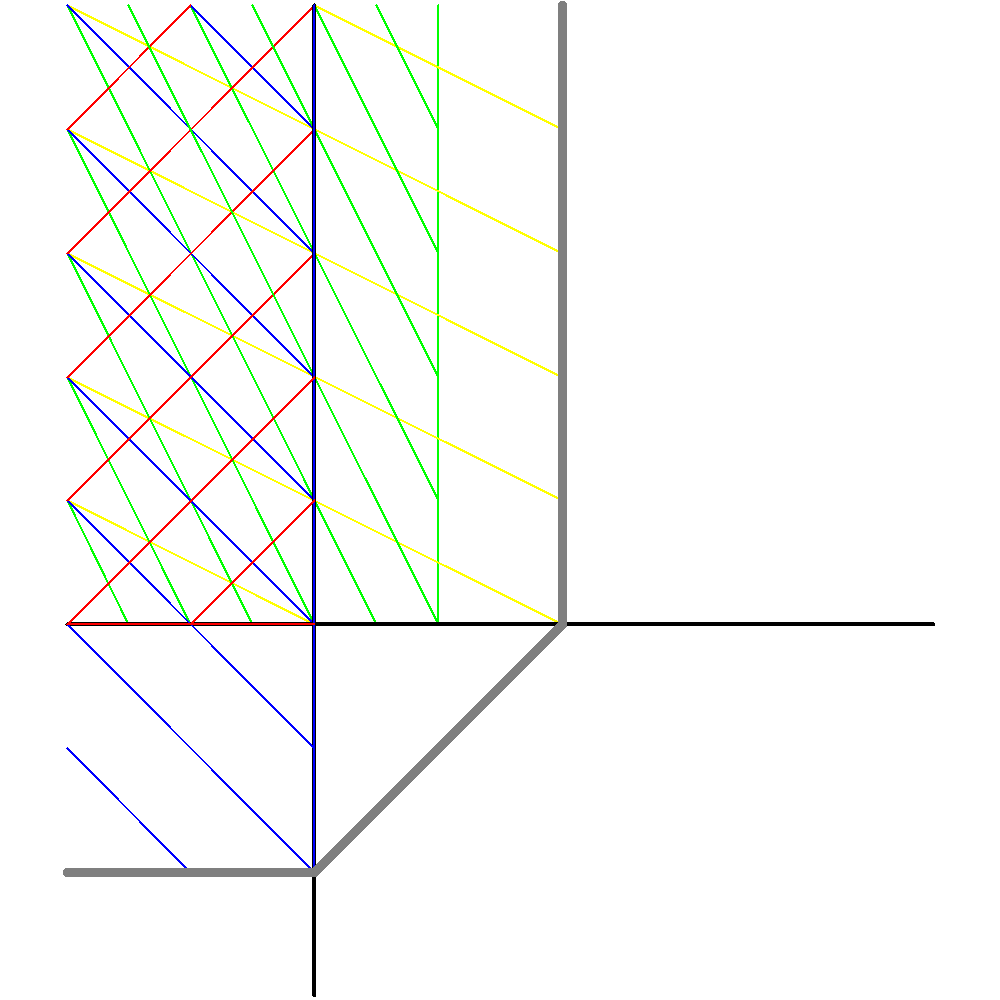
\includegraphics[width=6cm]{beispiele/img/a.png}
\end{center}
also $\slopes(P_a)=\{0\}$ also ist $P_a$ regulär singulär

% vim: set ft=tex :
 % nur ein slope: 1
%\subsection{zweites}
\[
  P_b=t\partial_t^2+2\partial_t-1
\]

$
P_b=t\partial_t^2+2\partial_t-1 \Rightarrow 
\begin{cases}
  k=2,l=1 & \Rightarrow u\leq l=2, v\geq l-k=-1\\
  k=1,l=0 & \Rightarrow u\leq 1, v\geq -1\\
  k=0,l=0 & \Rightarrow u\leq 0, v\geq 0\\
\end{cases}
$

\begin{center}
  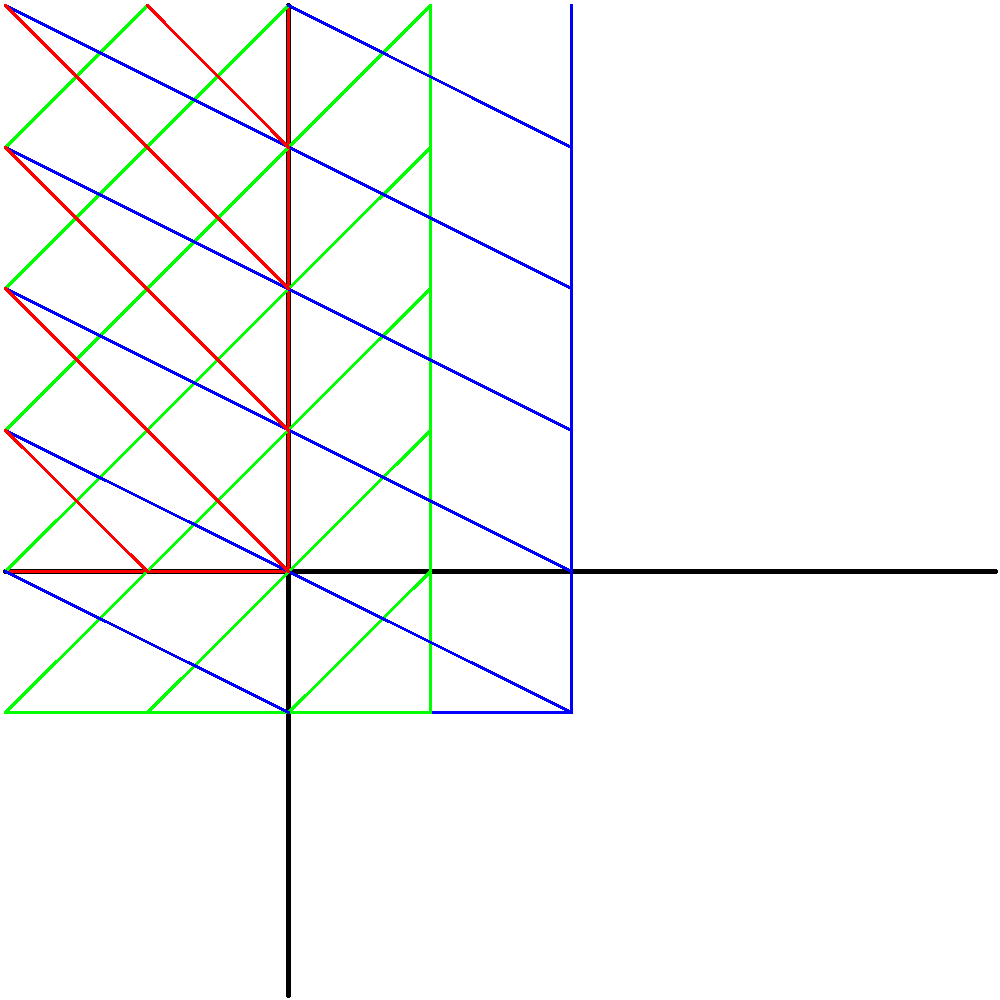
\includegraphics[width=6cm]{beispiele/img/b.png}
\end{center}
also $\slopes(P_b)=\{0\}$ also ist $P_b$ regulär singulär

% vim: set ft=tex :
 % regulär singulär
%\subsection{drittes}

\begin{comment}
  zula Barbara Seite 46
\end{comment}


\[
  P_c=t^2\partial_t+1
\]
$
P_c=t^2\partial_t+1
\Rightarrow
\begin{cases}
  k=1, l=2 & \Rightarrow u \leq 1, v \geq 1\\
  k=0, l=1 & \Rightarrow u \leq 0  v \geq 0\\
\end{cases}
$
\begin{center}
  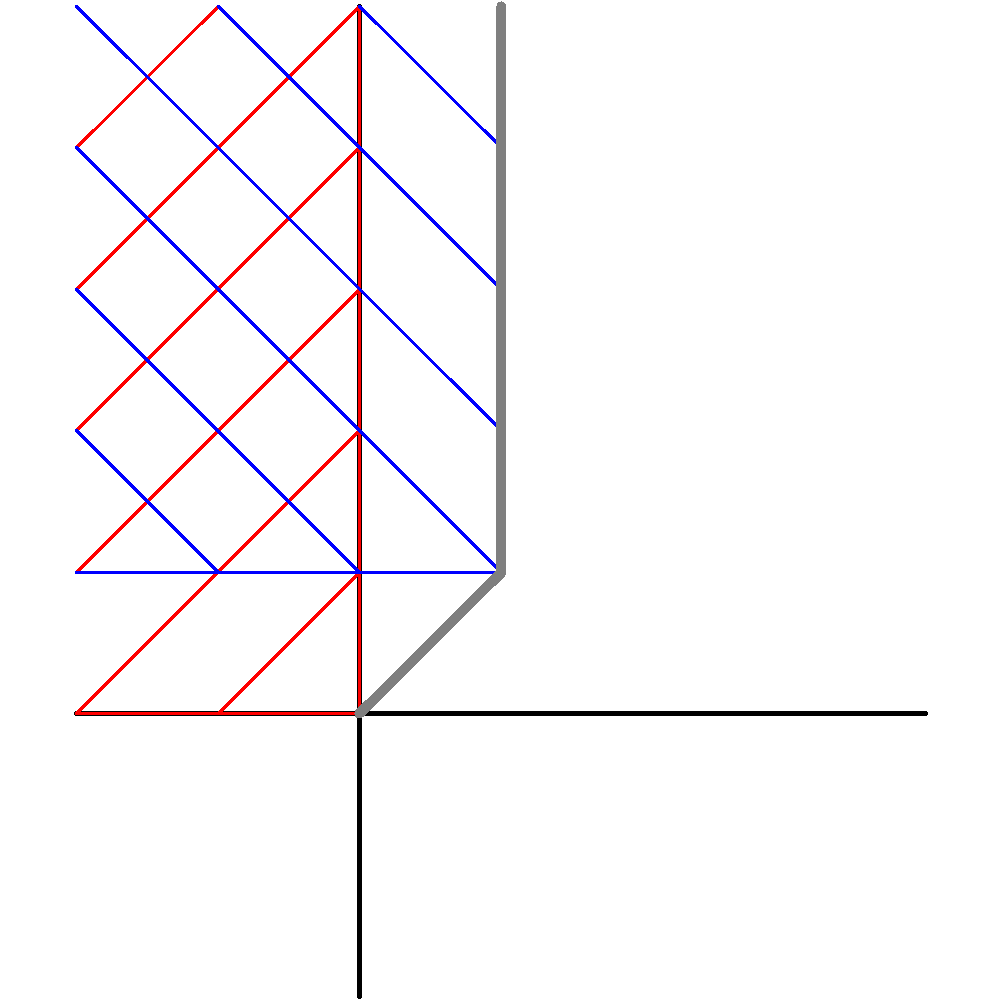
\includegraphics[width=6cm]{beispiele/img/c.png}
\end{center}

also $\slopes(P_c)=\{1\}$.

% vim:set ft=tex :
 % nur ein slope: 1
%\subsection{viertes}

\begin{comment}
  zula Barbara Seite 46
\end{comment}

\begin{comment}
  Original aus der Zula:
  \[
    P_d=-3t^{14}\partial_t^6+t^{11}(t+3)\partial_t^5 + 2t^8\partial_t^4
    -t^6(t^3+1)\partial_t^3 + t^4\partial_t
  \]

  $ P_d \Rightarrow
  \begin{cases}
    k=6,l=14 & \Rightarrow u\leq k=6, v\geq l-k=8\\
    k=5,l=12 & \Rightarrow u\leq 5, v\geq 7\\
    k=5,l=11 & \Rightarrow u\leq 5, v\geq 6\\
    k=4,l=8 & \Rightarrow u\leq 4, v\geq 4\\
    k=3,l=9 & \Rightarrow u\leq 3, v\geq 6\\
    k=3,l=6 & \Rightarrow u\leq 3, v\geq 3\\
    k=1,l=4 & \Rightarrow u\leq 1, v\geq 3\\
  \end{cases} $

  also ist Abbildung 5.8 auf seite 53 der zula falsch?
\end{comment}

\[
  P_d=-3t^{14}\partial_t^6+t^{11}(t+3)\partial_t^5 + 2t^8\partial_t^4
  -t^6(t^3+1)\partial_t^3 + t^3\partial_t
\]

$ P_d \Rightarrow
\begin{cases}
  k=6,l=14 & \Rightarrow u\leq k=6, v\geq l-k=8\\
  k=5,l=12 & \Rightarrow u\leq 5, v\geq 7\\
  k=5,l=11 & \Rightarrow u\leq 5, v\geq 6\\
  k=4,l=8 & \Rightarrow u\leq 4, v\geq 4\\
  k=3,l=9 & \Rightarrow u\leq 3, v\geq 6\\
  k=3,l=6 & \Rightarrow u\leq 3, v\geq 3\\
  k=1,l=3 & \Rightarrow u\leq 1, v\geq 2\\
\end{cases} $

\begin{center}
  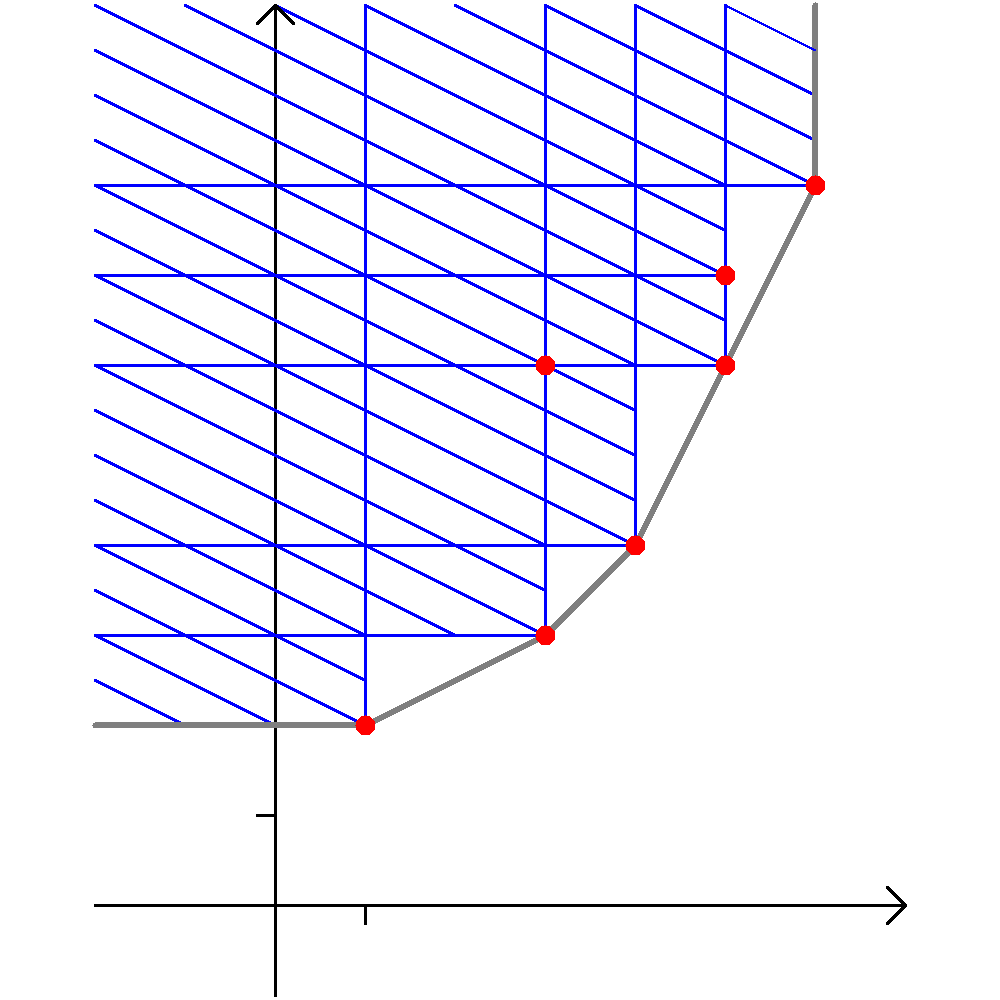
\includegraphics[width=6cm]{beispiele/img/d.png}
\end{center}
also $\slopes(P_b)=\{0,\frac{1}{2},1,2\}$ also ist $P_d$ irregulär singulär.\\
Offenbar ist der Hauptnenner der Steigugnen gleich $2$.\\
Betrachte also $\rho:t\mapsto u^2$\\
und erhalte: ???

% vim: set ft=tex :
 % zu kompliziert
%\subsection{bsp e}

\[
  P_e=t^4(t+1)\partial_t^4 + t\partial_t^2+\frac{1}{t}\partial_t+1
\]

\begin{center}
  \includegraphics[width=6cm]{beispiele/img/e.png}
\end{center}

also $\slopes(P_e)=\{0,\frac{2}{3}\}$

Dies gilt Analog für das einfachere:
\[
  \bar P_e=t^4\partial_t^4 +\frac{1}{t}\partial_t
\]

\begin{center}
  \includegraphics[width=6cm]{beispiele/img/bar_e.png}
\end{center}

% vim: set ft=tex :
 % verbesserte version: e_new
%Neuer versuch, ein geeignetes Beispiel zu finden

Hier soll ein einfaches Beispiel hergeleitet werden, an dem die Zerlegung nach
dem Levelt-Turittin-Theorem einmal explizit ausformuliert werden soll.

Beginne mit

\begin{minipage}[hbt]{0,49\textwidth}
  \[ t^4(t+1)\partial_t^4 + t\partial_t^2+\frac{1}{t}\partial_t+1 \]
\end{minipage}
\begin{minipage}[hbt]{0,49\textwidth}
  \begin{center}
    \includegraphics[width=3cm]{img/e.png}
  \end{center}
\end{minipage}

(von ZulaBarbara Seite 47)
und ignoriere zuerst die Terme, die zum Newton Polygon keinen Beitrag leisten

\begin{minipage}[hbt]{0,49\textwidth}
  \[ t^4\partial_t^4 +\frac{1}{t}\partial_t \]
\end{minipage}
\begin{minipage}[hbt]{0,49\textwidth}
  \begin{center}
    \includegraphics[width=3cm]{img/bar_e.png}
  \end{center}
\end{minipage}

multipliziere dieses mit $t$ und ändere aber dadurch den assoziierten
Meromorphen Zusammenhang nicht \cite[Chapter 5.1]{sabbah_cimpa90}

\begin{minipage}[hbt]{0,49\textwidth}
  \[ P:=t^5\partial_t^4 +\partial_t \]
\end{minipage}
\begin{minipage}[hbt]{0,49\textwidth}
  \begin{center} 
    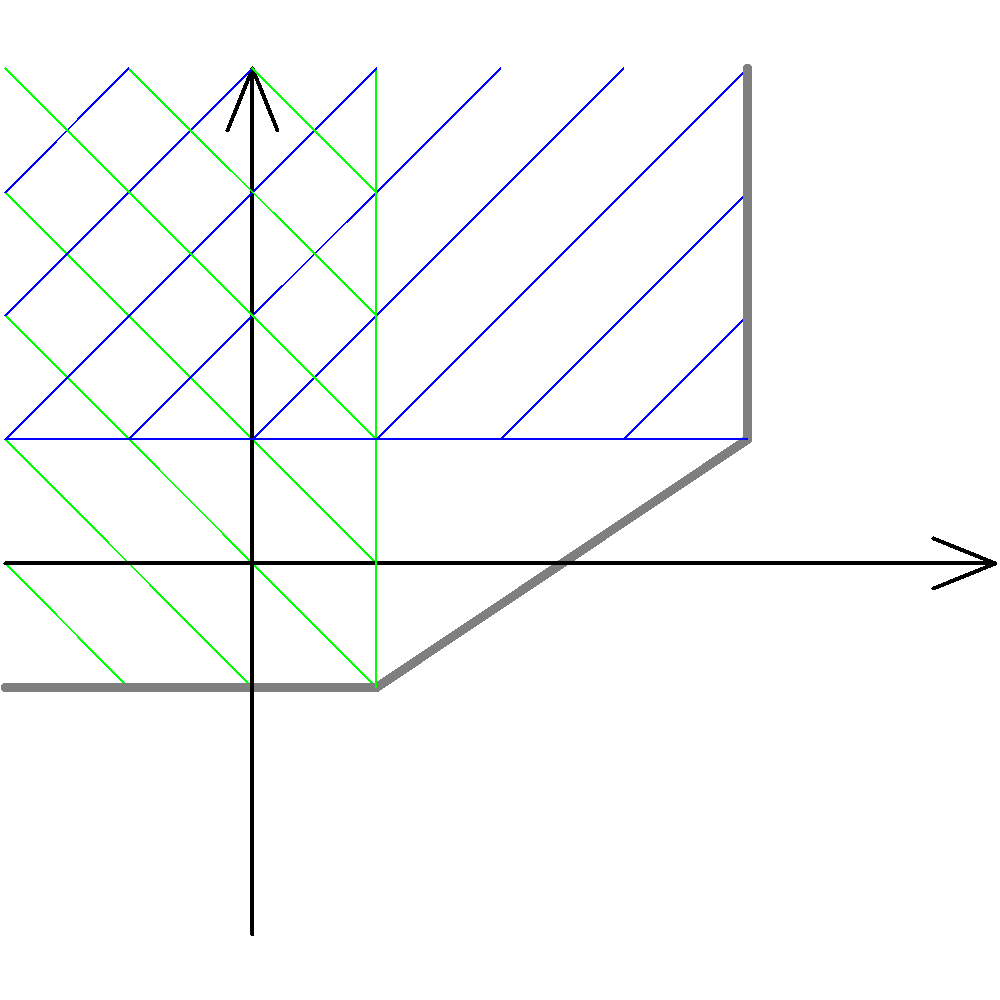
\includegraphics[width=3cm]{img/bar_e_times_x.png} 
  \end{center}
\end{minipage}

und es gilt $\slopes(P)=\{0,\frac{2}{3}\}$. Eliminiere als nächstes nun die
Brüche in den Slopes mittels einem geeignetem Pullback. Da hier der Hauptnenner
$3$ ist bietet sich $\rho:t\mapsto u^3$ für den Pullback an.
\begin{comment}
  Dieser Pullback Multipliziert (indirekt) die Slopes mit $3$,
  \textbf{Quelle?}\\ aber wie wendet man ihn (explizit) an?
\end{comment}

\[ \rho^+P=??? \]
welches die Slopes $\slopes(\rho^+P)=\{0,2\}\subset\Z$ hat. Schreibe nun dieses
$\rho^+P=Q\cdot R$ mit $P,Q\in\Cfu$ wobei gilt $\slopes(Q)=\{0\}$ und
$\slopes(R)=\{2\}$.

Also gilt:
\[
  \hat\cD/(\hat\cD\cdot\rho^+P)\cong
  \hat\cD/(\hat\cD\cdot Q) \oplus  \hat\cD/(\hat\cD\cdot R)
\]

% vim: set ft=tex :

\section{Meromorpher Zusammenhang der formal, aber nicht Konvergent, zerfällt}
%\begin{comment}
  %Quellen??
  %\[
    %\sum n!x^n
  %\]
%\end{comment}

% eine Übungsaufgabe aus sabbah_cimpba90 Seite 33
% 5.3.6
% 
% zwefällt formal aber NICHT konvergent

\subsection{beispiel von sabbah}

Sei $P=t(t\partial_t)^2+t\partial_t+\frac{1}{2}$

\begin{comment}
  \begin{enumerate}
      \item zeige $\cD/\cD\cdot P$ ist ein Meromorpher Zusammenhang.
      \item Zeichne das Newton Polygon von $P$ und finde eine formale
        Aufteilung von $\cM_{\hat{K}}$.
      \item Zeige $\cM$ kann nicht in eine direkte Summe von zwei $\cD$ modulen
        zerlegt werden, dazu:
        \begin{enumerate}
          \item Zeige das die Produktzerlegung
            \[ P=(t(t\partial_t)+v(t))\cdot(t\partial_t+u(t)) \,, \]
            mit $u,v\in\Cfu$, existiert.
          \item Berechne durch Induktion die Koeffizienten von $u$.
          \item Zeige dass $u \notin \C((u))$.
        \end{enumerate}
  \end{enumerate}
\end{comment}

\subsubsection{Schritt 1} Zeige das $\cD/\cD\cdot P$ einen Meromorphen
Zusammenhag Definiert.
\subsubsection{Schritt 2}
\begin{minipage}[hbt]{0,39\textwidth}
  \begin{align*}
   P &= t(t\partial_t)^2                + t\partial_t           + \frac{1}{2}\\
     &= tt(\partial_tt)\partial_t       + t\partial_t           + \frac{1}{2}\\
     &= t^2(t\partial_t + 1)\partial_t  + t\partial_t           + \frac{1}{2}\\
     &= t^3\partial_t^2                 + (t^2 + t)\partial_t   + \frac{1}{2}\\
  \end{align*}
\end{minipage}
\begin{minipage}[hbt]{0,59\textwidth}
  \begin{center}
    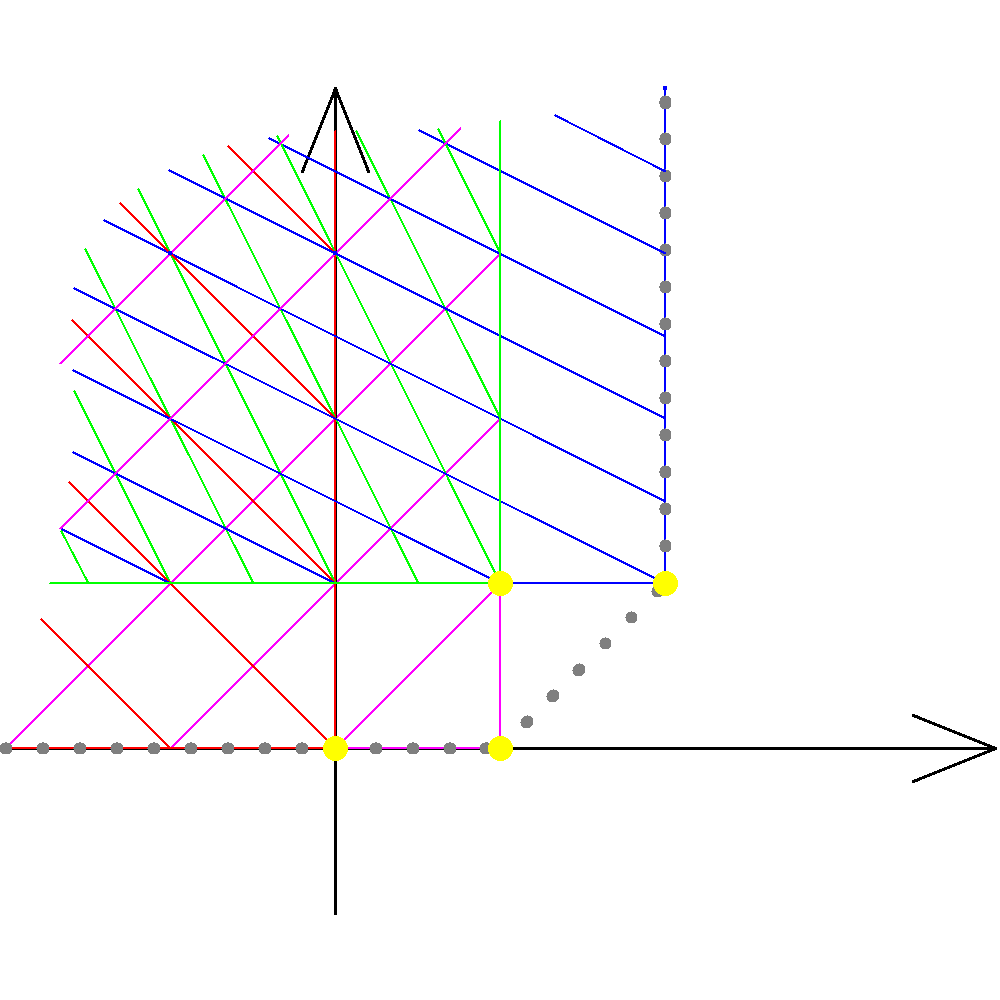
\includegraphics[width=6cm]{img/formal_a-2.png}
  \end{center}
\end{minipage}
Also mit $\slopes{P}=\{0,1\}$

\subsubsection{Schritt 3 a)}
\subsubsection{Schritt 3 b)}
\subsubsection{Schritt 3 c)}

% vim: set ft=tex :

%% entsteht aus b durch t --> 1/\tau

%hat nur einen Slope, also zerfällt nicht

%TODO: besserer Titel
\subsection{Beispiel ohne namen}
\begin{comment}
  Beginne mit
  \[ \tilde P=\tau\partial_\tau^2+2\partial_\tau-1 \]
  und gehe von $\tau$ über zu $t$ via $\tau\rightarrow\frac{1}{t}$:\\
  %TODO: rightarrow oder mapsto?
  \begin{itemize}
    \item was passiert mit der Ableitung $\partial_\tau$? Es gilt:
      \[
        \partial_\tau (f(\frac{1}{\tau}))=
        \partial_t(f)\cdot (-\frac{1}{\tau^2})=
        -\partial_t(f)\cdot t^2= %TODO: wegen klammerung?
        - t^2 \cdot \partial_t(f)
      \]
      also:
      \[
        \partial_\tau=-t^2\partial_t
        % stimmt das VZ?
      \]
    \item was ist $\partial_t(t^2\partial_t)$?
      \begin{align*}
        \partial_tt^2\partial_t &= (\partial_tt)t\partial_t\\
        &= (t\partial_t-1)t\partial_t\\
        &= t(\partial_tt)\partial_t-t\partial_t\\
        &= t(t\partial_t-1)\partial_t-t\partial_t\\
        &= t^2\partial_t^2-2t\partial_t\\
      \end{align*}
    \item was passiert mit $ \tilde P=\tau\partial_\tau^2+2\partial_\tau-1 $?
      \begin{align*}
        \tilde P &= \tau\partial_\tau^2+2\partial_\tau-1\\
        &\overset{\tau\rightarrow\frac{1}{t}}{\longrightarrow}
          \frac{1}{t}(-t^2\partial_t)^2+2(-t^2\partial_t)-1\\
        &= \frac{1}{t}t^2(\partial_t(t^2\partial_t))-2t^2\partial_t-1\\
        &= t(\partial_t(t^2\partial_t))-2t^2\partial_t-1\\
        &= t(t^2\partial_t^2-2t\partial_t)-2t^2\partial_t-1\\
        &= t^3\partial_t^2-4t^2\partial_t-1 =: P\\
      \end{align*}
  \end{itemize}
\end{comment}

Wir wollen nun den zum folgendem $P$ assoziierten Meromorphen Zusammenhang
betrachten:\\
\begin{minipage}[hbt]{0,39\textwidth}
  \[ P= t^3\partial_t^2-4t^2\partial_t-1 \]
  mit $ \slopes(P)=\{\frac{1}{2}\} $
\end{minipage}
\begin{minipage}[hbt]{0,59\textwidth}
  \begin{center}
    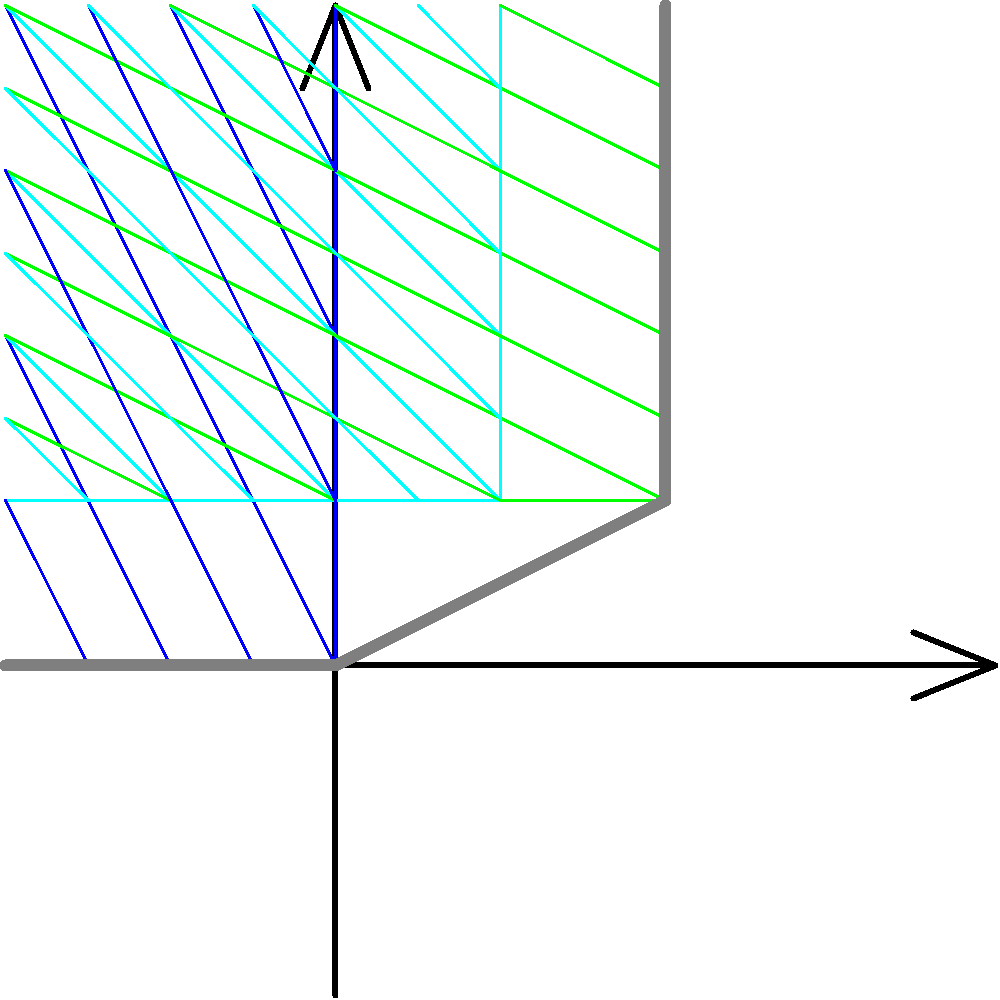
\includegraphics[width=6cm]{img/formal_b.png}
  \end{center}
\end{minipage}
%Es ist offensichtlich, dass $\slopes(P)=\{\frac{1}{2}\}$. 
Wir wollen ganzzahlige slopes haben, also wernde den pull-back
$\rho:t\rightarrow u^2$ an.

Zunächst ein paar nebenrechnungen: 
\begin{align*}
  \partial_t   &= \frac{1}{\rho'}\partial_u=\frac{1}{2u}\partial_u \\
  \partial_t^2 &= (\frac{1}{2u}\partial_u)^2\\
               &= \frac{1}{2u}(-\frac{1}{2u^2}\partial_u + 
                 \frac{1}{2u}\partial_u^2) \\
               &= -\frac{1}{4u^3}\partial_u+\frac{1}{4u^2}\partial_u^2 \\
\end{align*}
also
\begin{align*}
  \rho^+P &= u^6(-\frac{1}{4u^3}\partial_u+\frac{1}{4u^2}\partial_u^2)- 
            4u^{4}\frac{1}{2u}\partial_u-1\\
          &= -u^3\frac{1}{4u^3}\partial_u+\frac{1}{4}u^4\partial_u^2-
            4u^{3}\frac{1}{2}\partial_u-1\\
          &= \frac{1}{4}u^4\partial_u^2 -2\frac{1}{4}u^3\partial_u-1
\end{align*}

\begin{minipage}[hbt]{0,39\textwidth}
  \[ \rho^+P= \frac{1}{4}u^4\partial_u^2 -2\frac{1}{4}u^3\partial_u-1 \]
  mit $ \slopes(\rho^+P)=\{1\} $
\end{minipage}
\begin{minipage}[hbt]{0,59\textwidth}
  \begin{center}
    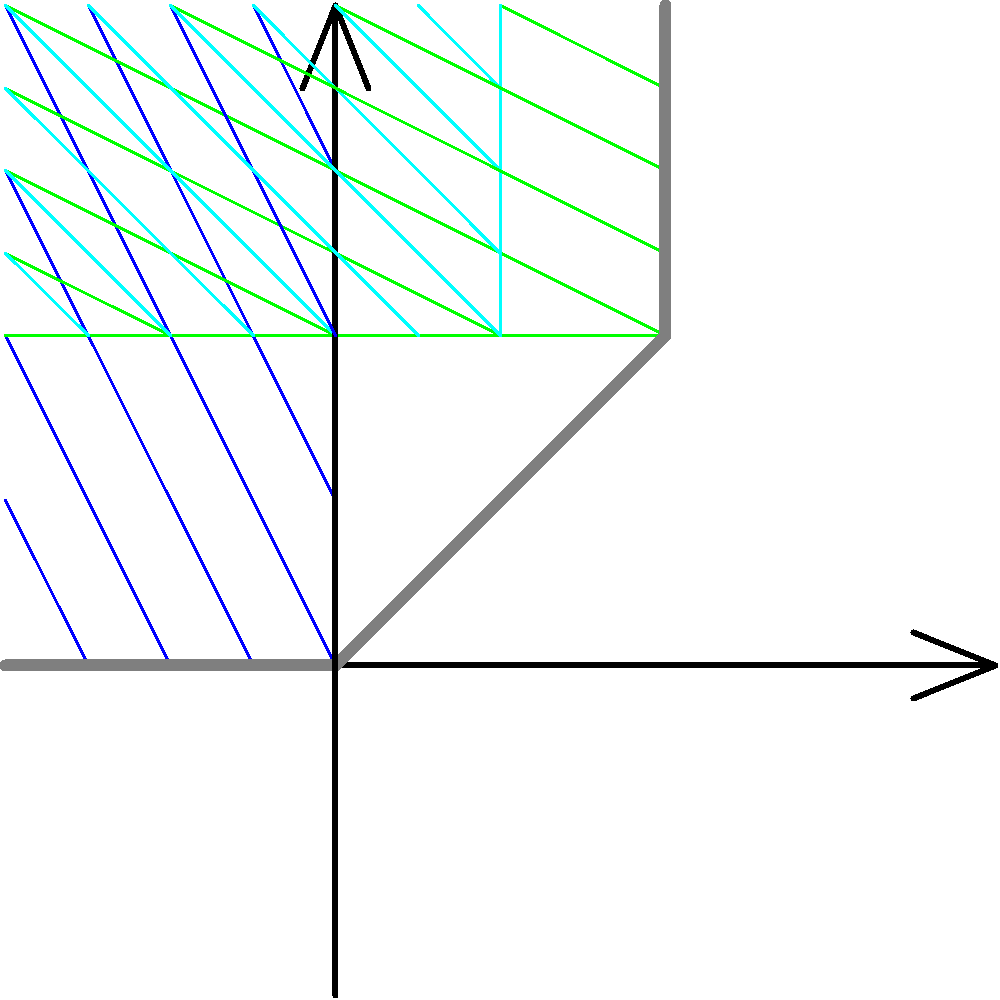
\includegraphics[width=6cm]{img/formal_b_pb.png}
  \end{center}
\end{minipage}

% vim: set ft=tex :


%\begin{comment}
  %Weiteres Beispiel:
  %\[
    %Sabbah\_Fourier-local.pdf \rightarrow 5.b.
  %\]
%\end{comment}

% vim: set ft=tex :


%%%%%%%%%%%%%%%%%%%%%%%%%%%%%%%%%%%%%%%%%%%%%%%%%%%%%%%%%%%%%%%%%%%%%
\appendix
\addcontentsline{toc}{chapter}{Anhang}

\begin{landscape}
  %\chapter{zur aufteilung in Lemma 2.4}
  \chapter{Aufteilung von ...}
  \label{chap:aufteilung}
  Sei $\phi\in u^{-1}\C[u^{-1}]$, so ist $\phi'=:\sum_{i=2}^N a_{-i}u^{-i}\in u^{-2}\C[u^{-1}]$ also 
  $u\phi'(u)=\sum_{i=1}^N a_{-i-1}u^{-i} \in u^{-1}\C[u^{-1}]$, welches wir zerlegen wollen.\\
  Zerlege also $u\phi'(u)=\sum_{j=0}^{p-1}u^j\psi_j(u^p)$
  mit $\psi_j\in\C[t^{-1}]$ für alle $j>0$ und $\psi_0\in
  t^{-1}\C[t^{-1}]$:\\
  \begin{center}
    \begin{tikzpicture} [descr/.style={fill=white,inner sep=2.5pt}]
    \matrix (m) [
      matrix of math nodes,
      row sep=1em,
      %column sep=-0.7em,
      text height=1.5ex,
      text depth=0.25ex]
    {
      & & & & & & & & & & & & & & \, \\
      u\phi'(u)= &
      a_{-2}u^{-1} &
      +...+ &
      a_{-p}u^{-(p-1)} &
      + &
      a_{-(p+1)}u^{-p} &
      + &
      a_{-(p+2)}u^{-(p+1)} &
      +...+ &
      a_{-2p}u^{-(2p-1)} &
      + &
      a_{-(2p+1)}u^{-2p} &
      + &
      a_{-(2p+3)}u^{-(2p+1)} &
      + ...  \\
      & & & & & & & & & & & & & & \, \\
    };

      \path[solid]
      (m-2-6) edge [bend left=20] node[descr]{$\psi_0(u^p)$} (m-2-12)
      (m-2-12)  edge [bend left=20] (m-1-15);

      \path[dotted]
      (m-2-4) edge [bend right=20] node[descr]{$u\psi_1(u^p)$} (m-2-10)
      (m-2-10)  edge [bend right=20] (m-3-15);

      \path[dashed]
      (m-2-2) edge [bend right=20] node[descr]{$u^{p-1}\psi_{p-1}(u^{p})$} (m-2-8)
      (m-2-8) edge [bend right=20] (m-2-14)
      (m-2-14) edge [bend right=20] (m-3-15);
    \end{tikzpicture}
  \end{center}
  also:\\
  \begin{align*}
    \psi_0(u^p) &= a_{-(p+1)}u^{-p}+a_{-(2p+1)}u^{-2p}+...\\
    \psi_1(u^p) &= a_{-p}u^{-p}+a_{-2p}u^{2p}+...\\
    & \vdots & \\
    \psi_{p-1}(u^p) &= a_{-2}u^p+a_{-(p+2)}u^{2p}+...\\
  \end{align*}
\end{landscape}


\nocite{*}
%\bibliographystyle{dinat}
%\bibliographystyle{plain}
\bibliographystyle{amsalpha}
\bibliography{main}

\end{document}
